\documentclass[a4paper]{article}

\usepackage[utf8]{inputenc}
\usepackage[portuguese]{babel}
\usepackage{a4wide}
\usepackage[pdftex]{hyperref}
\usepackage{graphicx}
\usepackage{wrapfig}
\usepackage{amsmath}
\usepackage{caption}
\usepackage{subcaption}
\usepackage{tikz}
\usepackage{pgfplots}
\pgfplotsset{compat=1.10}
\usepgfplotslibrary{fillbetween}
\usepackage{pgfplots}
\usetikzlibrary{patterns}
\usepackage{float}
\usepackage{lmodern}



\begin{document}

\begin{titlepage}
\begin{center}



\includegraphics[width=0.4\textwidth]{logo}\\[0.3cm]

{\large Universidade do Minho - Escola de Engenharia}\\[0.5cm]

{\large Relatório do trabalho prático de Desenvolvimento de Sistemas de Software}\\[0.5cm]



% Title
\rule{\linewidth}{0.5mm} \\[0.4cm]
{ \huge \bfseries Sistema de Gestão de Turnos Práticos \\[0.4cm] }
\rule{\linewidth}{0.5mm} \\[1.5cm]

% Author and supervisor
\noindent
\begin{minipage}{0.4\textwidth}
  \begin{flushleft} \large
    \emph{Autores :}\\
    Diana Costa \textsc{(A78985)}\\
    
\includegraphics[width=1.5cm]{diana}\break
    Marcos Pereira \textsc{(A79116)}\\
    
\includegraphics[width=1.5cm]{marcos}\break
    Sérgio Oliveira\textsc{(A77730)}\\
    
\includegraphics[width=1.5cm]{sergio}\break
    Vítor Castro\textsc{(A77870)}\\
    
\includegraphics[width=1.5cm]{vitor}\break
  \end{flushleft}
\end{minipage}%
\vfill

% Bottom of the page
{\large Versão 1.0 \\ \today}

\end{center}
\end{titlepage}


\begin{abstract}

\hspace{3mm}Neste relatório será feita uma abordagem ao projeto de Desenvolvimento de Sistemas de Software ao qual está associado o desenvolvimento de um programa, em Java, responsável pela gestão dos turnos de um curso. Assim, este documento apresenta, detalhadamente, a perspetiva tomada pelo grupo em relação ao problema proposto pela equipa docente de DSS.

\end{abstract}

\pagebreak
\tableofcontents

\pagebreak
\section{Introdução}
\label{sec:1}

\hspace{3mm}Este trabalho foi elaborado no âmbito da Unidade Curricular de Desenvolvimento de Sistemas de Software, do 3º ano do Mestrado Integrado em Engenharia Informática, com vista à implementação de um sistema de gestão de alunos e horários do curso.

Esta aplicação deverá suportar o registo dos alunos e professores, sendo gerida pela Direção de Curso, que deverá criar Turnos e associar os mesmos às Unidades Curriculares existentes. Cada UC deverá ter um docente responsável. Os docentes registados lecionarão um ou mais turnos, bem como os alunos estarão inscritos a um ou mais turnos, de acordo com as cadeiras em que se registem, aquando do seu registo.

O processo de levantamento de requisitos foi fácil, uma vez que vai ser replicada uma plataforma aplicada no ano letivo 2017/2018, denominada de SWAP, cujo objetivo é exatamente o mesmo que a aplicação a realizar. No entanto, a aplicação a desenvolver difere no modo como são propostas trocas em relação à aplicação original. De facto, na SWAP, um aluno pode propôr uma troca a outro, mas esta será única (para cada UC). Na visão do grupo, o melhor sistema será o de um género de bolsa de trocas, em que os alunos demonstram a sua vontade de mudar do turno que têm atualmente para um turno determinado por eles, sendo que todos os outros alunos poderão efetuar a troca, se esta for de encontro às suas necessidades.

Neste relatório, a parte inicial corresponderá à primeira fase do trabalho, em que se procedeu à elaboração do Modelo de Domínio, dos Use Cases e respetivas especificações e do Protótipo de Interface. Este Diagramas permitiram fazer a especificação das necessidades levantadas em relação à aplicação.
Depois, serão exibidos os restantes Diagramas pedidos, a saber: de Classes, de Sequência, de Máquinas de Estado, de Atividades, de Packages e, por fim, de Instalação. Em alguns destes diagramas, será possível verificar as mudanças que ocorreram entre a sua conceção no início do desenvolvimento e o fim.

Por fim, será possível ver o resultado final da aplicação quanto à sua interface, bem como se implementou \textit{DAOs} e o \textit{parsing} dos dados em JSON para a BD, tudo necessidades encontradas no levantamento dos requisitos. O grupo almeja desenvolver a atribuição automática de turnos, sendo que este aspeto será abordado na Conclusão.

\section{Problema}
\label{sec:2}

\hspace{3mm}

\hspace{3mm}Pretende-se desenvolver um sistema que atribui turnos (e, deste modo, um horário) aos alunos do curso e possibilita a ocorrência de trocas entre estes. As trocas estão condicionadas pela existência de dois alunos interessados em trocar de turno, no caso de pertencerem ao regime normal, e são feitas sem condicionalismos no caso do aluno ser trabalhador estudante. O programa deverá ser capaz, também, de permitir que os docentes responsáveis de cada UC possam inscrever alunos em turnos assim como removê-los. O diretor de curso terá acesso a todas as funcionalidades pelo que além das funcionalidades do docente, conseguirá também criar turnos, criar UCs, registar docentes responsáveis no sistema e atribuir estes docentes às UCs respetivas.

\clearpage
\section{Solução}
\label{sec:3}


\hspace{3mm}A solução apresentada baseia-se na UML - \emph{Unified Modeling Language} - linguagem útil na elaboração, modelação e documentação da estrutura de projetos de software e de sistemas orientados a objetos. Portanto, auxilia os \emph{developers} de programas a visualizarem os seus sistemas através de diagramas padronizados.

Baseia-se também num programa desenvolvido em JAVA que, à partida, consegue atingir todas as funcionalidades pretendidas pelo enunciado, com a exceção da sobreposição de turnos a qual não foi verificada nem assegurada pelo grupo de trabalho.

\pagebreak
\subsection{Modelo de Domínio}
\hspace{3mm}O modelo de domínio analisa o problema de uma perspetiva concetual e é uma aproximação da representação gráfica das classes do programa e dos seus atributos, assim como o relacionamento entre estas.

O modelo de domínio gerado a partir dos requisitos propostos é o mostrado abaixo. As principais entidades identificadas são aluno, turno, e troca, o que é explicado pelo principal foco da aplicação, as trocas de turnos, envolverem estas principalmente. As restantes entidades completam o esquema, uma vez que um turno tem de pertencer a uma UC, que por sua vez é gerida por um docente. A direção de curso gere a maioria das entidades, e um aluno pode ter um regime de estudante ou de trabalhador estudante.
Em seguida, apresentam-se dois diagramas, sendo o primeiro relativo à fase inicial do projeto e o segundo à final.

\begin{figure}[H]
\centering
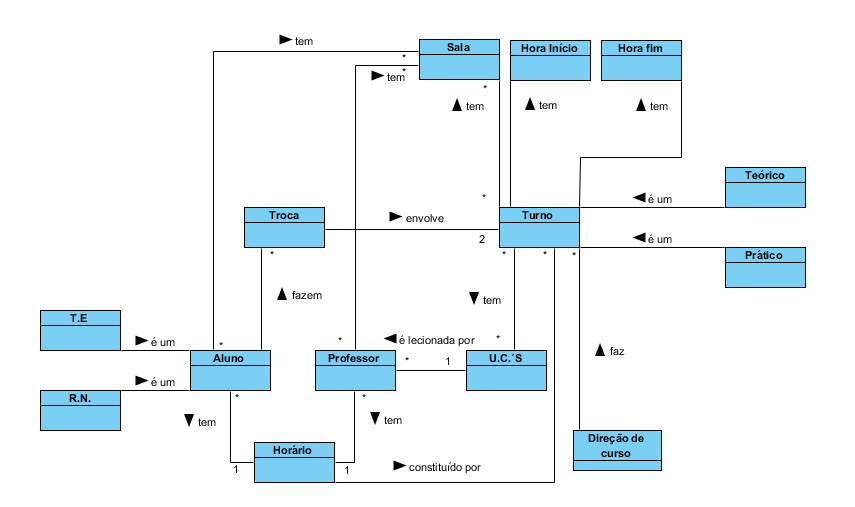
\includegraphics[width=14cm]{ModeloDominioAntigo}
\caption{Modelo de Domínio da 1ª fase do projeto}
\label{}
\end{figure}

\begin{figure}[H]
\centering
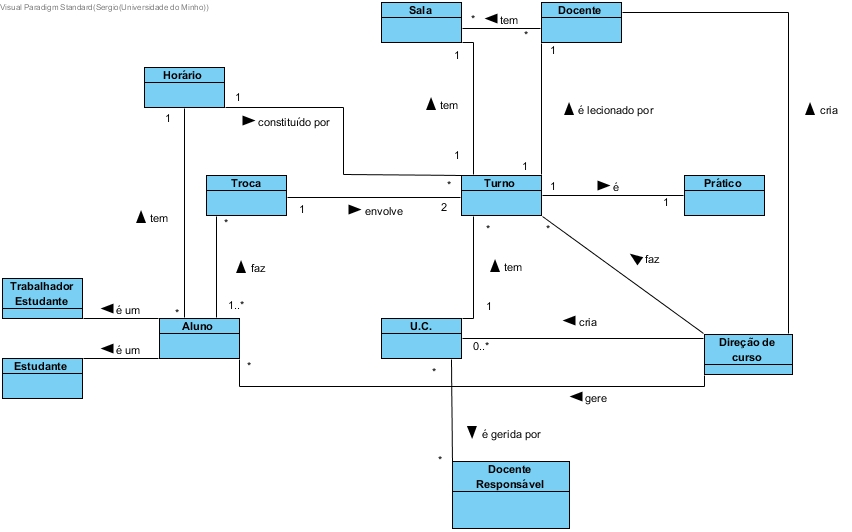
\includegraphics[width=14cm]{ModeloDominio}
\caption{Modelo de Domínio final}
\label{}
\end{figure}

\clearpage
\subsection{Diagrama de Use Cases}
\hspace{3mm}O esquema de Use Cases é o diagrama que mostra o que o programa faz do ponto de vista do utilizador, ou seja, consegue mostrar as principais funcionalidades do sistema e as suas interações com os atores do mesmo. Por isso, os diagramas de use case são compostos por atores (utilizadores do sistema), por use cases (funcionalidade) e pelas comunicações entre atores e use case.

O grupo decidiu implementar uma bolsa de trocas, na qual todos os alunos teriam igualdade de oportunidade de troca, e assumiu-se que, caso houvesse um trabalhador-estudante, esse aluno poderia realizar a troca automaticamente

No que toca aos docentes (Docente-Responsável e Docente), depois de refletir sobre a pertinência de haver uma entidade Docente (que não responsável da UC) e sabendo que a única interação que poderia ter seria a de registar faltas, decidiu-se pela sua retirada. O motivo desta decisão prende-se pelo objetivo da Plataforma a ser desenvolvida, a saber, resolver um problema de atribuição de horários, e não pela marcação de faltas (apesar das mesmas terem uma implicação no horário de um Aluno, caso este falte a mais de 25 por cento das aulas). Deste modo, assume-se que as faltas serão contabilizadas tal como o são no momento e, a dada altura, o Docente-Responsável aperceber-se-á que determinado aluno deve ser removido do turno, funcionalidade essa que está disponível.

A Direção de Curso foi criada com o objetivo de poder ser o controlador principal de todo o sistema, sendo que pode fazer qualquer operação sem problema.

\begin{figure}[H]
\centering
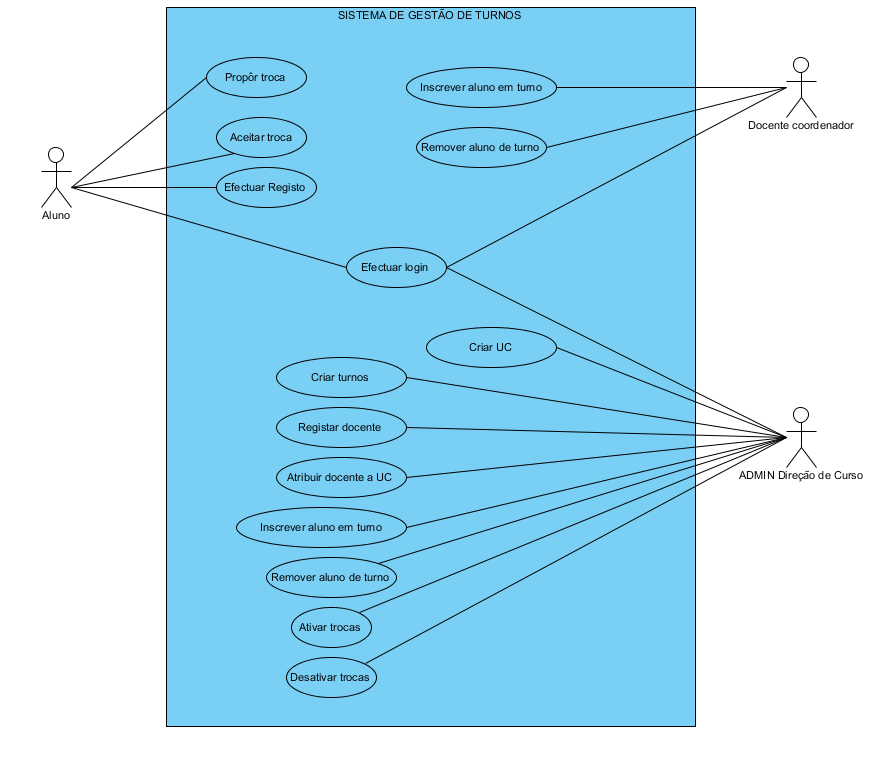
\includegraphics[width=14cm]{usecases}
\caption{Diagrama de Use Cases}
\label{}
\end{figure}

\clearpage
\subsection{Especificação textual dos Use Cases}
\hspace{3mm}Dado que um cenário é uma sequência de passos da interação entre ator e sistema, então a especificação textual dos casos de uso é um documento que descreve os vários cenários possíveis entre as comunicações de um mesmo objetivo ou funcionalidade. Apenas serão explicados alguns dos Use Cases (considerados mais importantes), uma vez que a sua explanação é suficiente para a compreensão de todo o problema.

\subsubsection{Criar UC}
\hspace{3mm}Responsabilidade do DC, que deve inserir a UC no sistema, preenchendo os campos necessários à caracterização da mesma. O sistema verifica a inserção dos dados e cria a UC, caso tudo esteja correto.

\begin{figure}[H]
\centering
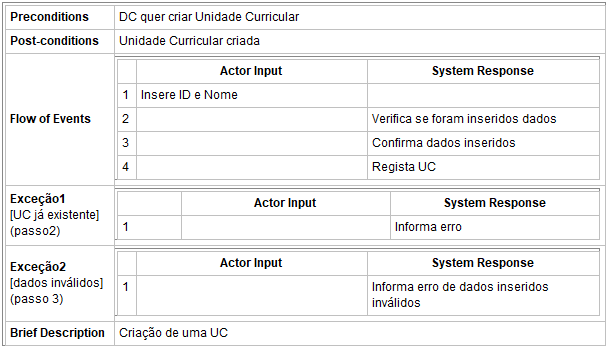
\includegraphics[width=14cm]{UCCriarUCADMIN}
\caption{Especificação textual do use case "Criar UC"}
\label{}
\end{figure}

\clearpage
\subsubsection{Criar turnos}
\hspace{3mm}Responsabilidade do DC, que deve selecionar a UC para a qual quer criar turnos e, deve preencher os campos relativos a ID do turno, número máximo de alunos no turno, nome do professor e sala de aula. O sistema verifica se foi tudo preenchido e cria o turno.

\begin{figure}[H]
\centering
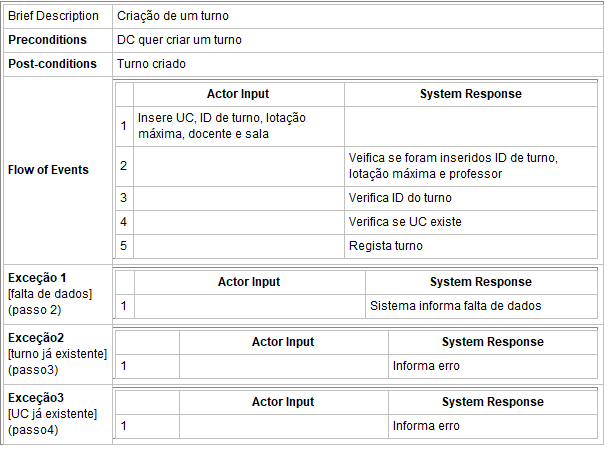
\includegraphics[width=14cm]{UCCriarTurnosADMIN}
\caption{Especificação textual do use case "Criar turnos"}
\label{}
\end{figure}

\clearpage
\subsubsection{Registar docente}
\hspace{3mm}Responsabilidade do DC, o qual deve fornecer os dados relativos a nome do docente a ser criado, bem como o seu ID e a sua password, que serão utilizados futuramente, para que este consiga fazer login no sistema como professor responsável. O sistema verifica se os campos foram preenchidos e cria o docente.

\begin{figure}[H]
\centering
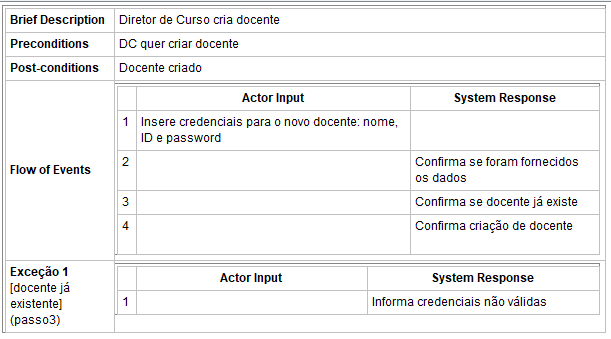
\includegraphics[width=14cm]{UCRegistarDocenteADMIN}
\caption{Especificação textual do use case "Registar docente"}
\label{}
\end{figure}

\subsubsection{Atribuir docente a UC}
\hspace{3mm}O DC depois de criar um docente, deve associar este à UC da qual é responsável. Por isso, deve selecionar o docente pretendido da lista de docentes registados no sistema e deve selecionar a UC. O sistema faz as devidas verificações e associa o docente à unidade curricular.

\begin{figure}[H]
\centering
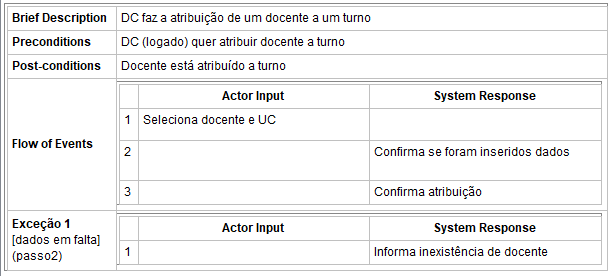
\includegraphics[width=14cm]{UCAtribuirDocenteAUcADMIN}
\caption{Atribuir docente a UC"}
\label{}
\end{figure}

\subsubsection{Inscrever aluno em turno[ADMIN]}
\hspace{3mm}O DC poderá inscrever um aluno num turno do sistema. Para isso, deve selecionar a unidade curricular, o aluno em questão (é necessário que o aluno esteja inscrito na disciplina), o turno de origem do aluno (é possível que não tenha turno também) e o turno de destino. O sistema fará a inscrição.


\begin{figure}[H]
\centering
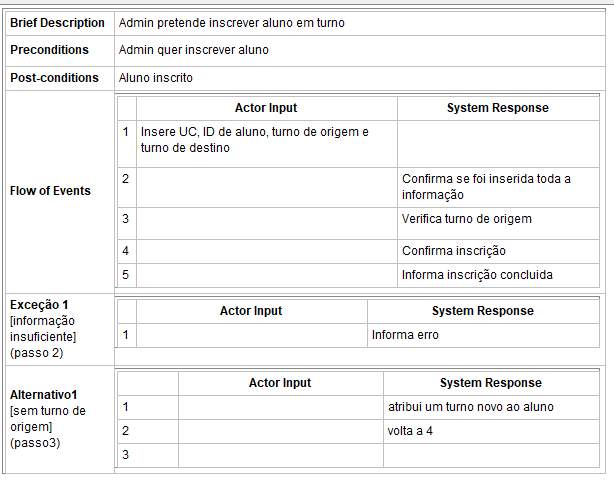
\includegraphics[width=14cm]{UCInscreverAlunoEmTurnoADMIN}
\caption{Especificação textual do use case "Inscrever aluno em turno" pelo Admin}
\label{}
\end{figure}

\clearpage
\subsubsection{Remover aluno de turno[ADMIN]}
\hspace{3mm}Responsabilidade atribuída ao diretor de curso, que apenas terá de selecionar a unidade curricular onde pretende efetuar a remoção. De seguida, seleciona o turno no qual o aluno está inscrito e deve selecionar o aluno em questão. O sistema fará a remoção, se tudo for bem sucedido.

\begin{figure}[H]
\centering
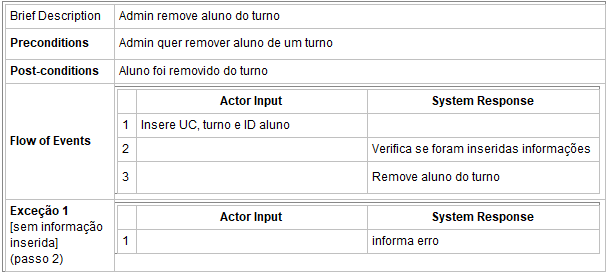
\includegraphics[width=14cm]{UCRemoverAlunoDeTurnoADMIN}
\caption{Especificação textual do use case "Remover aluno de turno" pelo Admin}
\label{}
\end{figure}

\subsubsection{Ativar Trocas}
\hspace{3mm}Responsabilidade do DC que será capaz de ativar o sistema de trocas quando assim entender. Aplicável no início do semestre.

\begin{figure}[H]
\centering
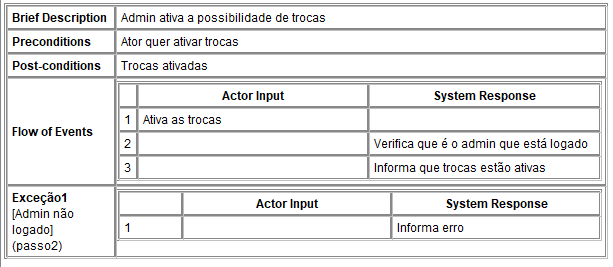
\includegraphics[width=14cm]{UCAtivarTrocasADMIN}
\caption{Especificação textual do use case "Ativar trocas"}
\label{}
\end{figure}

\clearpage
\subsubsection{Desativar Trocas}
\hspace{3mm}Responsabilidade do DC que poderá desativar o sistema de trocas. Aplicável no fim do prazo estabelecido para inscrições.

\begin{figure}[H]
\centering
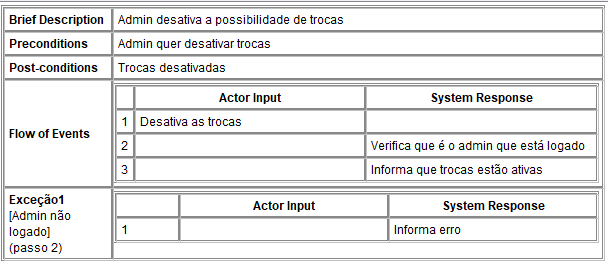
\includegraphics[width=14cm]{UCDesativarTrocas}
\caption{Especificação textual do use case "Desativar Trocas"}
\label{}
\end{figure}

\subsubsection{Efetuar Login}
\hspace{3mm}O utilizador (Aluno, Docente ou DC) faz login. As suas credenciais são verificadas e, caso aprovadas, terá acesso à sua área pessoal de acordo com os seus privilégios. O login é negado caso o utilizador seja inexistente ou a password não seja a correta.

\begin{figure}[H]
\centering
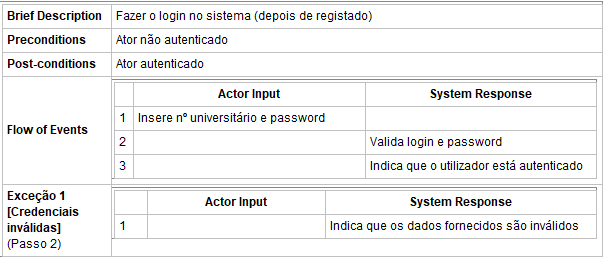
\includegraphics[width=14cm]{UCEfetuarLogin}
\caption{Especificação textual do use case "Efetuar Login"}
\label{}
\end{figure}

\clearpage
\subsubsection{Efetuar Registo}
\hspace{3mm}Só efetuado por alunos que, durante o registo, devem registar um identificador (número mecanográfico, por exemplo) e uma password, o seu regime e também as UCs a que se querem inscrever. É feita a verificação de inserção dos dados.

\begin{figure}[H]
\centering
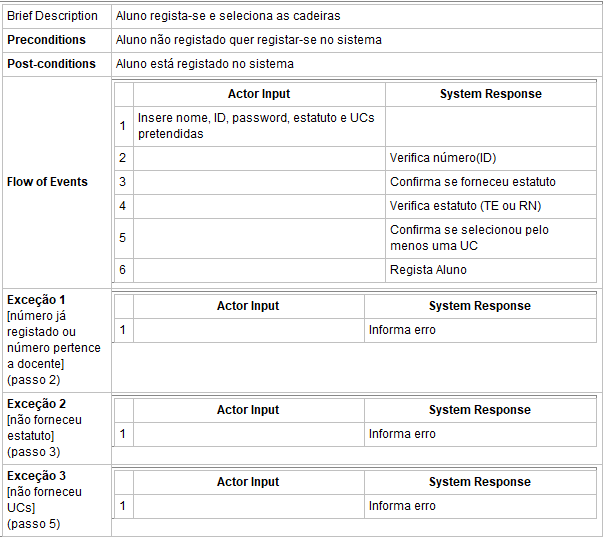
\includegraphics[width=14cm]{UCEfetuarRegisto}
\caption{Especificação textual do use case "EfetuarRegisto"}
\label{}
\end{figure}

\clearpage
\subsubsection{Inscreve aluno em turno[DOCENTE]}
\hspace{3mm}Tarefa atribuída ao Docente-Responsável que, segundo uma política de utilização responsável, não terá qualquer problema em adicionar qualquer aluno ao turno desejado (da UC que leciona). Deverá selecionar o aluno em questão (é necessário que o aluno esteja inscrito na disciplina), o turno de origem do aluno (é possível que não tenha turno também) e o turno de destino. O sistema fará a inscrição.

\begin{figure}[H]
\centering
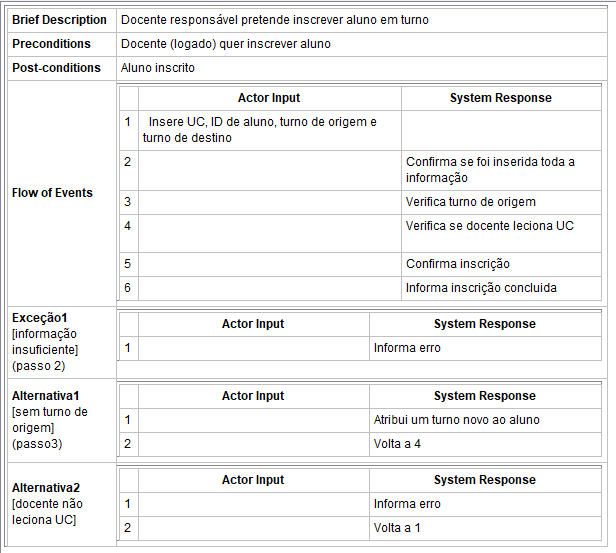
\includegraphics[width=14cm]{UCInscreverAlunoEmTurnoDOCENTE}
\caption{Especificação textual do use case "Inscrever aluno em turno" pelo docente}
\label{}
\end{figure}

\clearpage
\subsubsection{Remover aluno de turno[DOCENTE]}
\hspace{3mm}Responsabilidade atribuída ao Docente-Responsável, que apenas deverá de selecionar o turno no qual o aluno está inscrito e deve selecionar o aluno em questão. O sistema fará a remoção, se tudo for bem sucedido.

\begin{figure}[H]
\centering
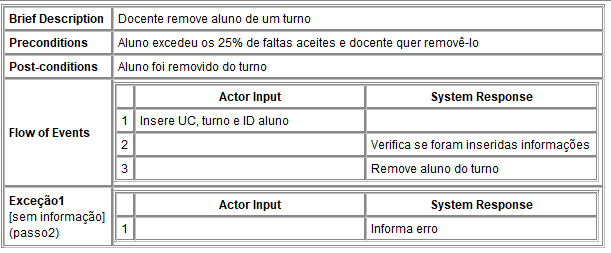
\includegraphics[width=14cm]{UCRemoverAlunoDeTurnoDOCENTE}
\caption{Especificação textual do use case "Remover aluno de turno" pelo docente}
\label{}
\end{figure}

\clearpage
\subsubsection{Propôr Troca}
\hspace{3mm}Só efetuado por alunos sendo que, após seleção do turno e UC desejados, é lançada essa proposta para a bolsa de trocas e a oferta ficará à espera de ser aceite por parte de outro aluno. Neste ponto, no caso de a oferta ter sido feita por um trabalhador estudante, então a oferta não é colocada na bolsa de trocas e é automaticamente aceite pelo sistema, isto se a sala do turno tiver ainda lugares disponíveis.

\begin{figure}[H]
\centering
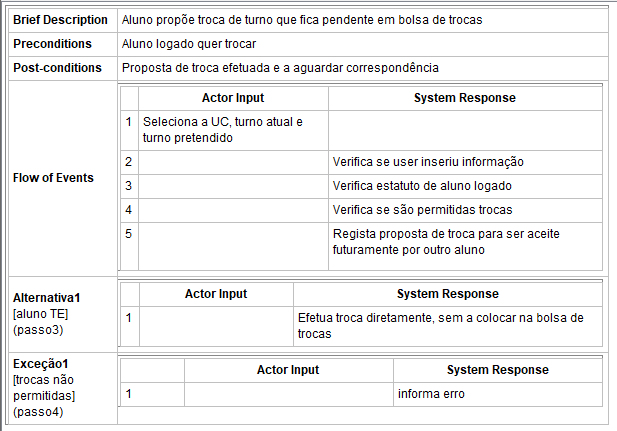
\includegraphics[width=14cm]{UCProporTroca}
\caption{Especificação textual do use case "Propôr troca"}
\label{}
\end{figure}

\clearpage
\subsubsection{Aceitar Troca}
\hspace{3mm}Só efetuado por alunos sendo que, após seleção do turno e UC desejados, é lançada essa proposta para a bolsa de trocas. Posteriormente, outro aluno consultará a bolsa de trocas e aceitará ou não a oferta. Para aceitar, é necessário, de facto, que seja possível, ou seja, o seu turno atual deverá corresponder ao turno pretendido pelo estudante que fez a oferta. O sistema faz esta verificação automaticamente pelo que o botão de aceitar a oferta, só aparecerá na interface do aluno, se houver possibilidade.

\begin{figure}[H]
\centering
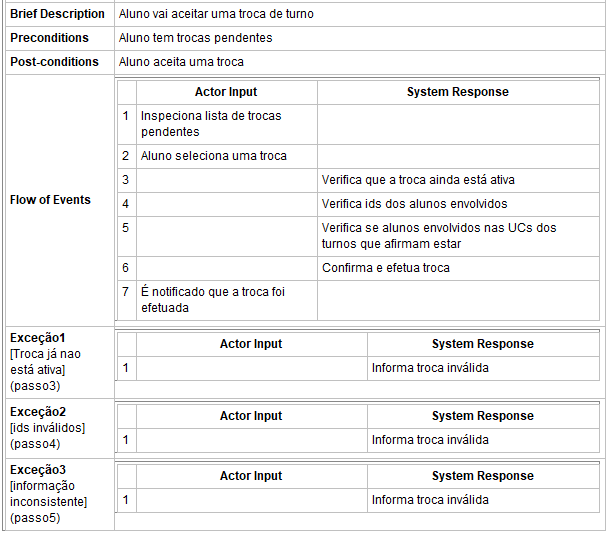
\includegraphics[width=14cm]{UCAceitarTroca}
\caption{Especificação textual do use case "Aceitar troca"}
\label{}
\end{figure}

\pagebreak

\subsection{Model View Controller}
\hspace{3mm}Antes de dar início ao desenvolvimento do programa em si, e por ser uma aplicação com recurso a uma interface gráfica, foi necessário alocar algum tempo à organização das classes de maneira a haver uma separação de preocupações (\emph{separation of concerns}).

O paradigma MVC (\emph{Model View Controller}) já é bastante popular no que toca à separação da lógica de negócio de uma aplicação da sua interface, assim como da partilha de informação entre estes. Nas aulas foi-nos sugerida a utilização do paradigma \emph{Observer} em Java, onde basicamente uma classe é definida como \emph{Observable}, e uma ou várias outras registam-se como observadoras. Quando a classe \emph{Observable} emite uma notificação, é invocado um método nas classes observadoras, onde o evento deve ser analisado e a reação correspondente deve ser efetuada.

Nesta fase de análise, identificamos um problema com a utilização deste paradigma: à medida que fosse adicionada funcionalidade à interface, o método que receberia os eventos da \emph{View} (caso a \emph{View} fosse o \emph{Observable}) acabaria por crescer de uma maneira descontrolada, tornando-se numa espécie de \emph{God Method}.

Como alternativa, e com base no nosso background em \emph{javascript} com \emph{callbacks} e \emph{promises}, encontramos uma solução mais moderna (apenas se tornou disponível no Java 8) que consiste no envio de referências a métodos para a \emph{View}, que seriam depois chamados quando ocorressem eventos. Por exemplo:

\vspace{3mm}



Para o evento de registo, a \emph{View} teria um método chamado \emph{onRegister}, que recebe um \emph{Consumer}. Um \emph{Consumer} é uma referência a um método que recebe um único parâmetro de um tipo T.

O \emph{Controller} teria um método também chamado \emph{onRegister}, que recebe um parâmetro do tipo T mencionado anteriormente. Dentro de um outro método, chamado \emph{attachToView}, são enviadas para a \emph{View} todas as referências necessárias para serem recebidas notificações de eventos, incluindo o agora criado \emph{onRegister}. Dentro do \emph{attachToView}, teríamos a linha \emph{this.view.onRegister(this::onRegister)}. A \emph{View} guarda a referência ao método numa variável local \emph{registrationListener} (ou numa lista com vários \emph{registrationListeners}), e invoca esses ouvintes assim que houver um registo.

\vspace{3mm}

Para que isto seja possível, é necessário que o \emph{Controller} possua uma referência à instância da \emph{View} a ser utilizada, assim como uma referência ao \emph{Model} para invocar os métodos da camada de negócio necessários.

Estas referências são passadas aquando da inicialização da aplicação pela classe principal \emph{ScheduleManager}.

Com esta solução, conseguimos manter os métodos relacionados com eventos da \emph{View} pequenos e fáceis de ler, assim como alcançar uma total independência entre o \emph{Model} e a \emph{View}, apenas o \emph{Controller} sabendo da existência de ambos e sendo responsável pela cooperação entre os dois.

\begin{figure}[h]
\centering
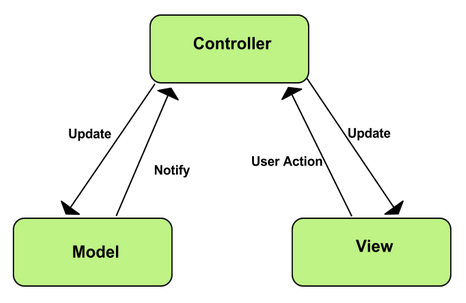
\includegraphics[width=0.5\textwidth]{mvcflavor}
\caption{Um diagrama que ajuda a esclarecer o nosso \emph{flavor} de MVC}
\label{}
\end{figure}

\subsection{Diagrama de Classes}

Aqui se apresentam os diagramas de classes, antes e depois da aplicação dos \emph{DAOs}.

\subsubsection{PRÉ-DAOs}
\begin{figure}[H]
\centering
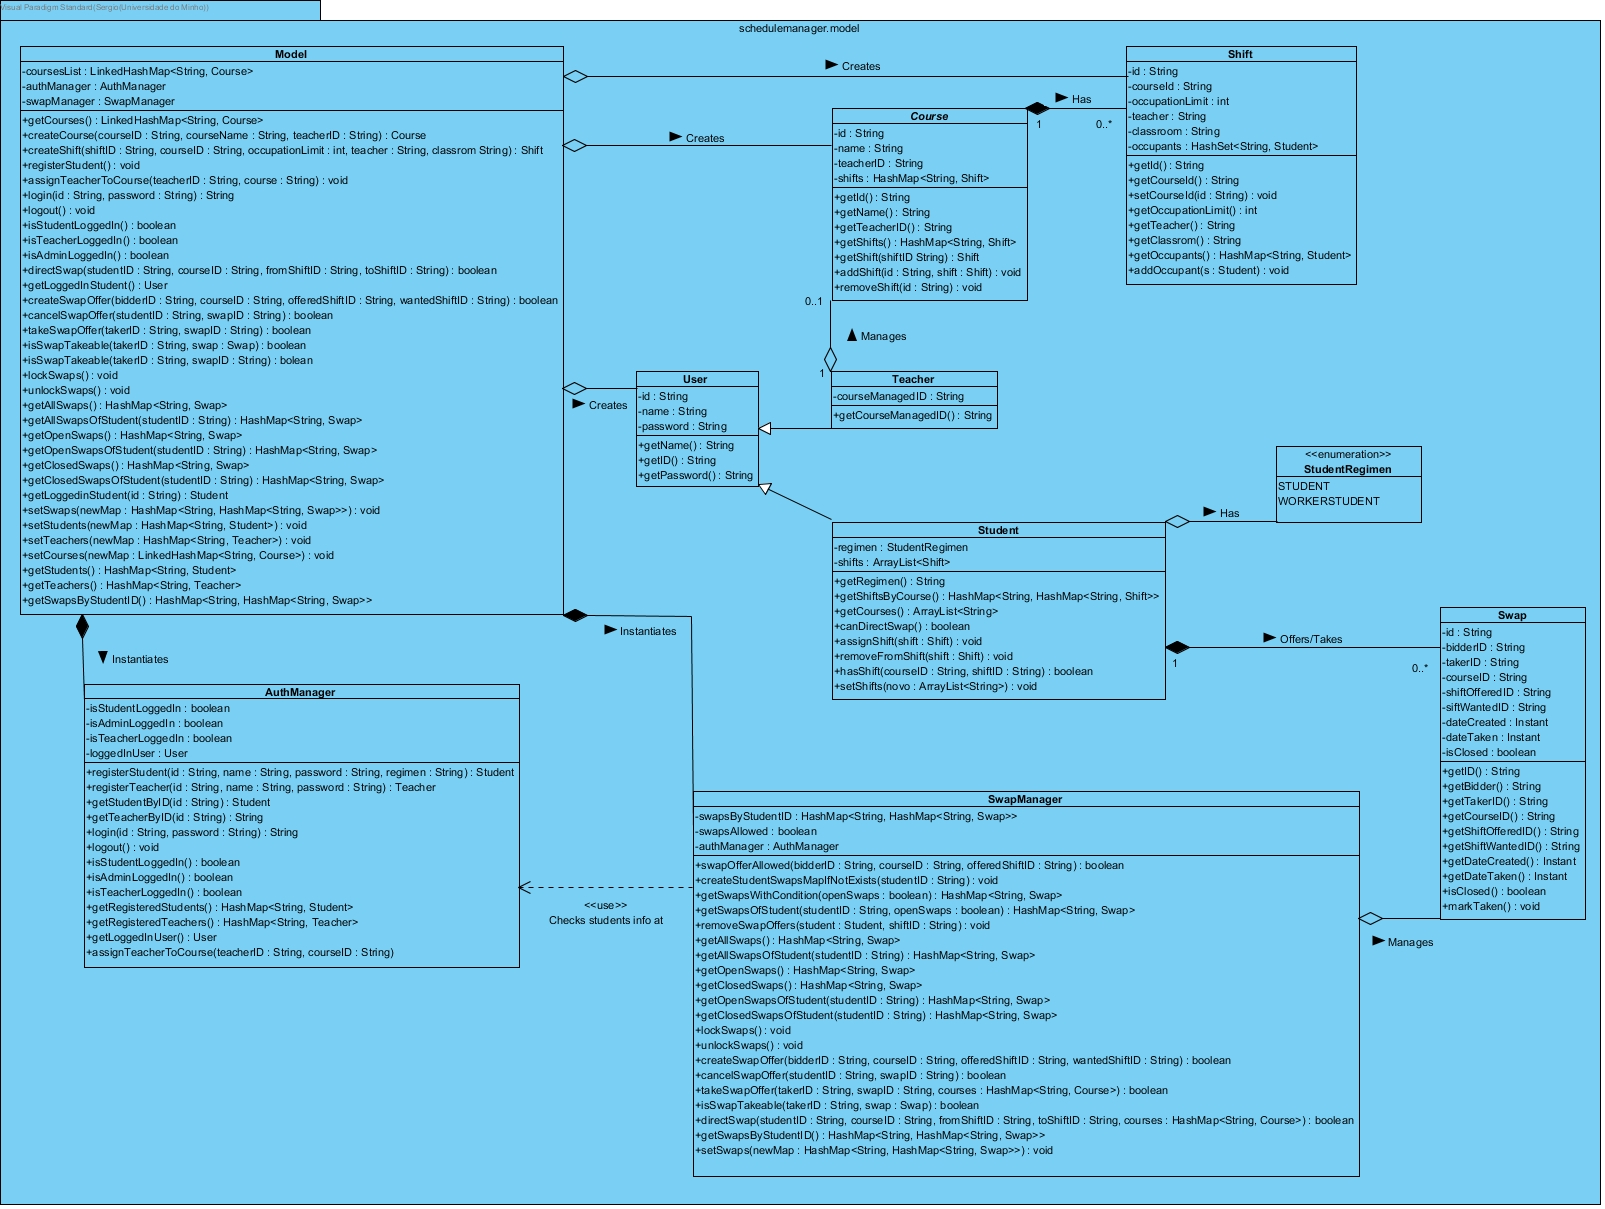
\includegraphics[width=14cm]{DiagramaClasses}
\caption{Diagrama de classes sem DAOs}
\label{}
\end{figure}

\subsubsection{PÓS-DAOs}
\begin{figure}[H]
\centering
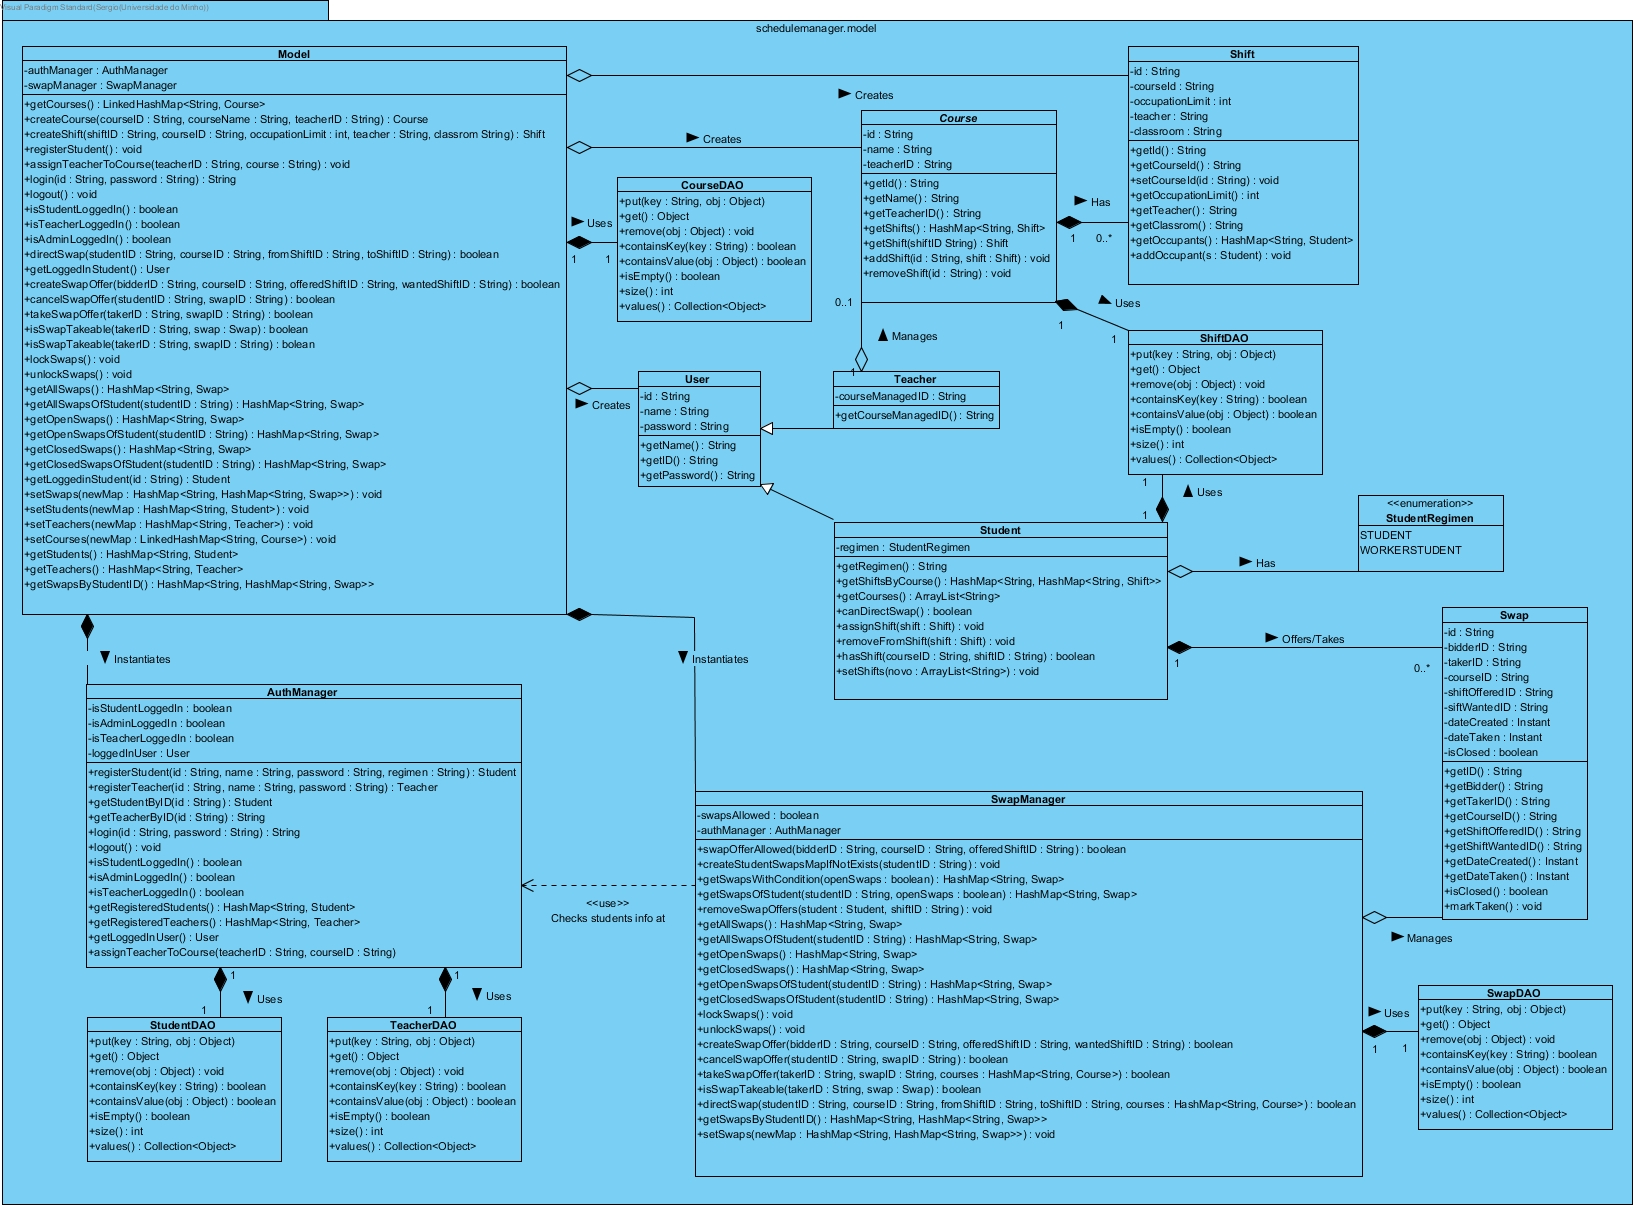
\includegraphics[width=14cm]{DiagramaClassesDAO}
\caption{Diagrama de classes com DAOs}
\label{}
\end{figure}

\clearpage
\subsection{Diagramas de Sequência}

Nos diagramas seguintes, faz-se a representação da troca de mensagens entre os diversos objetos ou instâncias de classe, necessária para que se consigam obter os resultados aos quais é preciso responder com sucesso.

Decidiu-se que não valia a pena aprofundar a ligação ou as mensagens entre View e Controller, uma vez que nos iríamos desviar do foco principal. Além disso, o funcionamento do MVC foi já explicado. Assim, foi introduzido "(...)" entre as duas lifelines.
Além do mais, todos os diagramas apresentam, no início, as self messages: "data.get(0)", "data.get(1)",... 
Na verdade, não correspondem a self messages, mas como a estrutura de dados "data" é um parâmetro do método, de onde vem a informações dos "Consumers" da \emph{view}, decidiu-se que ficaria melhor representar por \emph{self messages}.


\subsubsection{Criar UC[ADMIN]}

\begin{figure}[H]
\centering
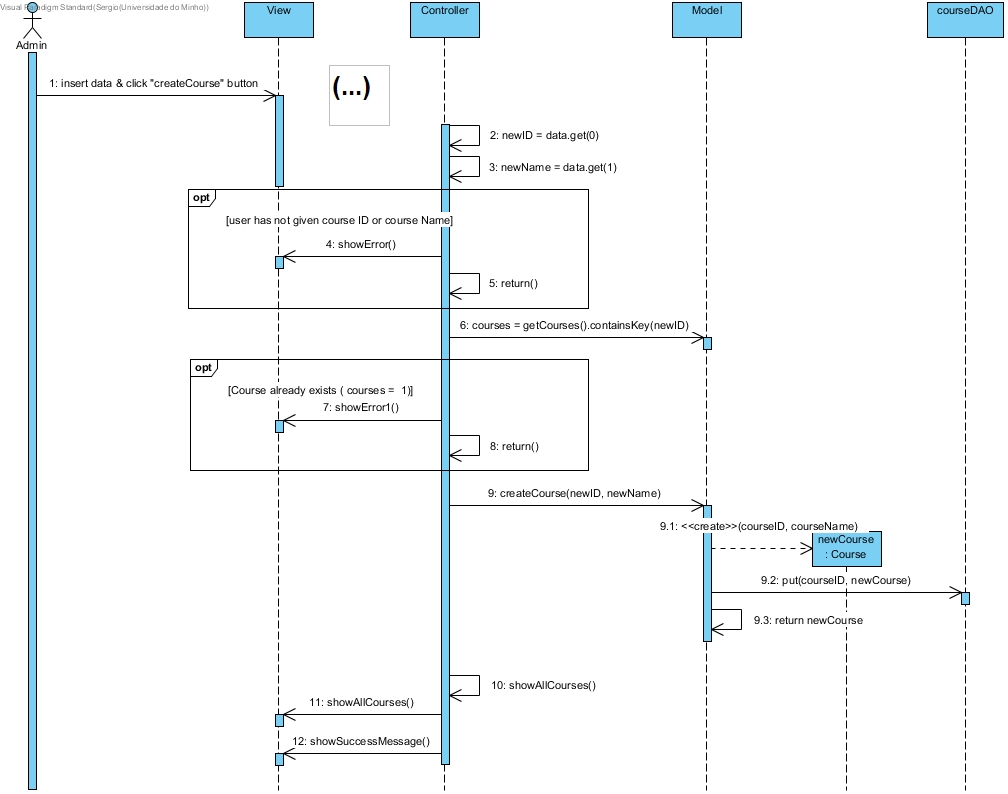
\includegraphics[width=14cm]{SEQcriarUC}
\caption{Diagrama de sequência para criação de UC pelo ADMIN}
\label{}
\end{figure}

\subsubsection{Criar turnos[ADMIN]}

\begin{figure}[H]
\centering
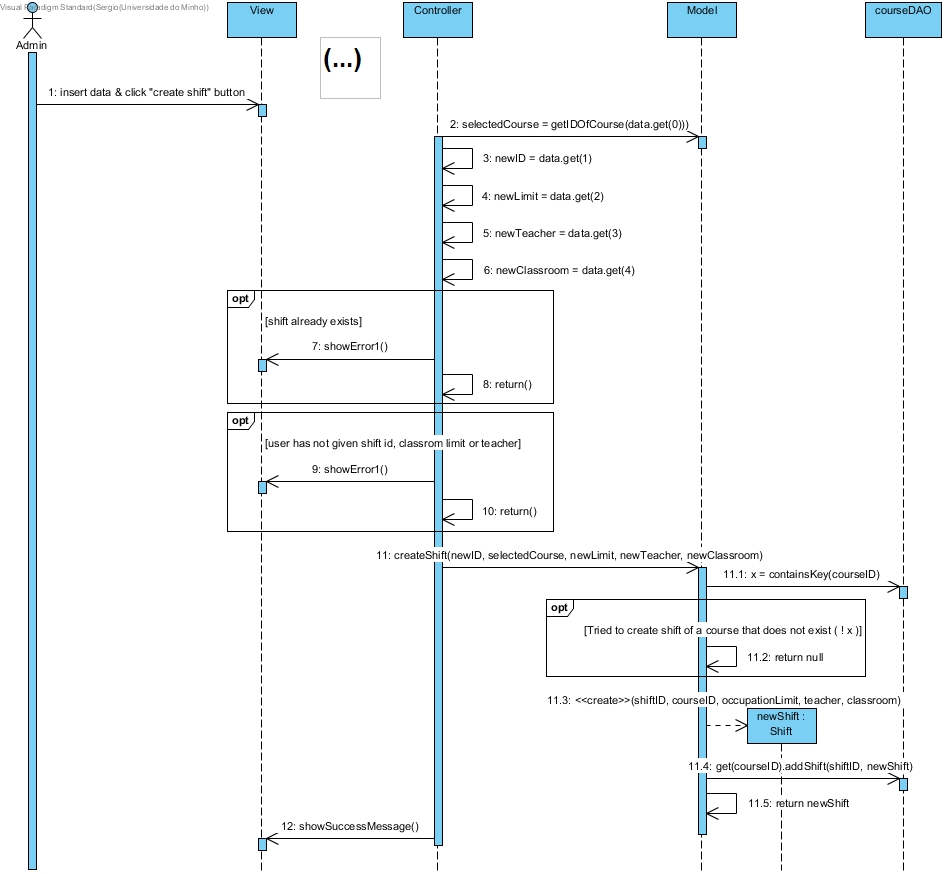
\includegraphics[width=14cm]{SEQcriarTurnos}
\caption{Diagrama de sequência para criação de turno pelo ADMIN}
\label{}
\end{figure}

\subsubsection{Registar docente}

\begin{figure}[H]
\centering
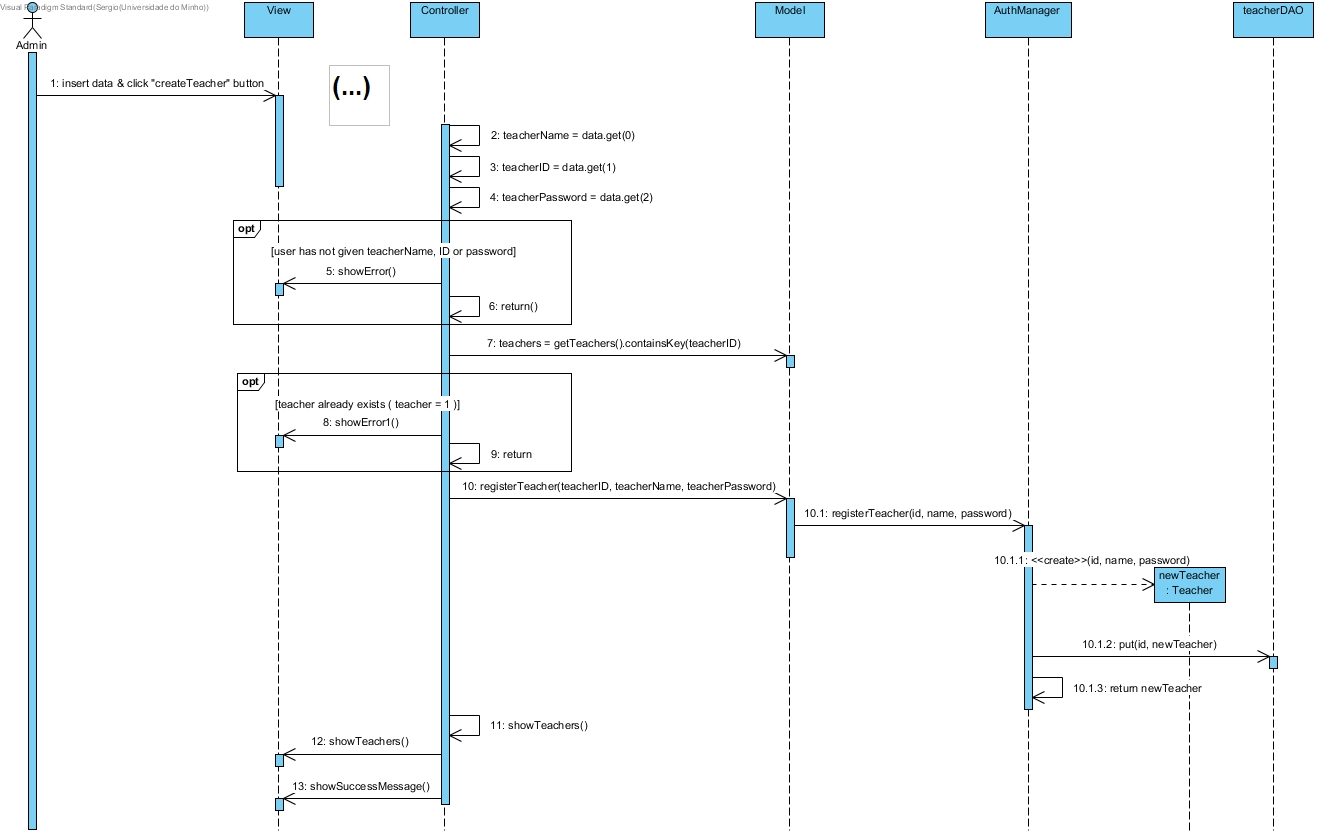
\includegraphics[width=14cm]{SEQregistarDocente}
\caption{Diagrama de sequência para registo de Docente pelo ADMIN}
\label{}
\end{figure}

\subsubsection{Atribuir docente a UC}

\begin{figure}[H]
\centering
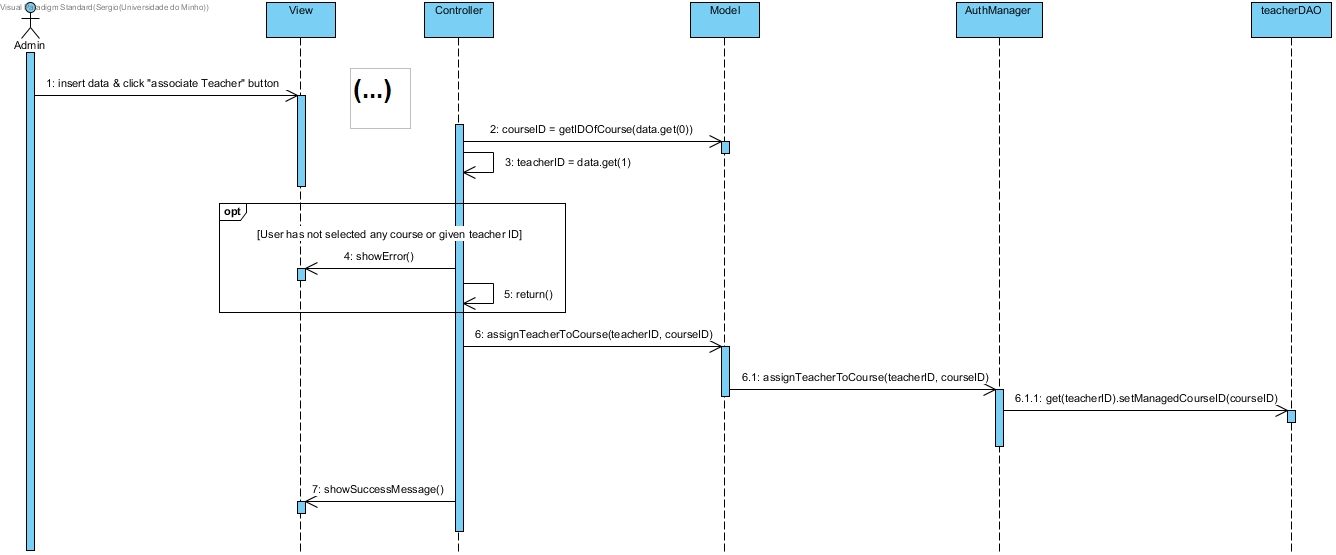
\includegraphics[width=14cm]{SEQAssociarDocenteAUC}
\caption{Diagrama de sequência para atribuição de docente a UC pelo ADMIN}
\label{}
\end{figure}

\subsubsection{Inscrever aluno em turno[ADMIN]}

\begin{figure}[H]
\centering
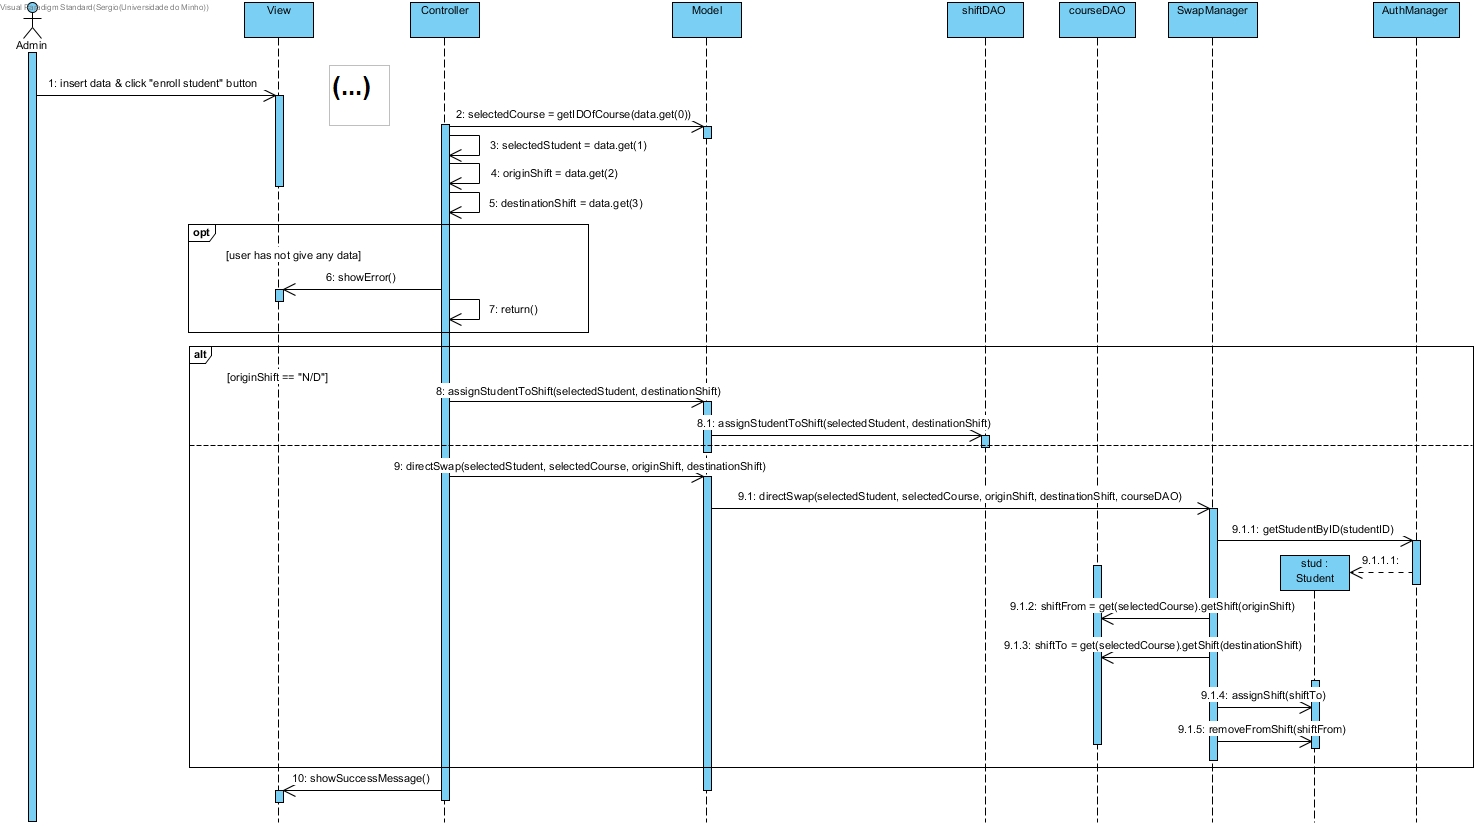
\includegraphics[width=14cm]{SEQInscreverAlunoTurno(peloAdmin)}
\caption{Diagrama de sequência para inscrição de um aluno num turno, pelo ADMIN}
\label{}
\end{figure}

\subsubsection{Remover aluno de turno[ADMIN]}

\begin{figure}[H]
\centering
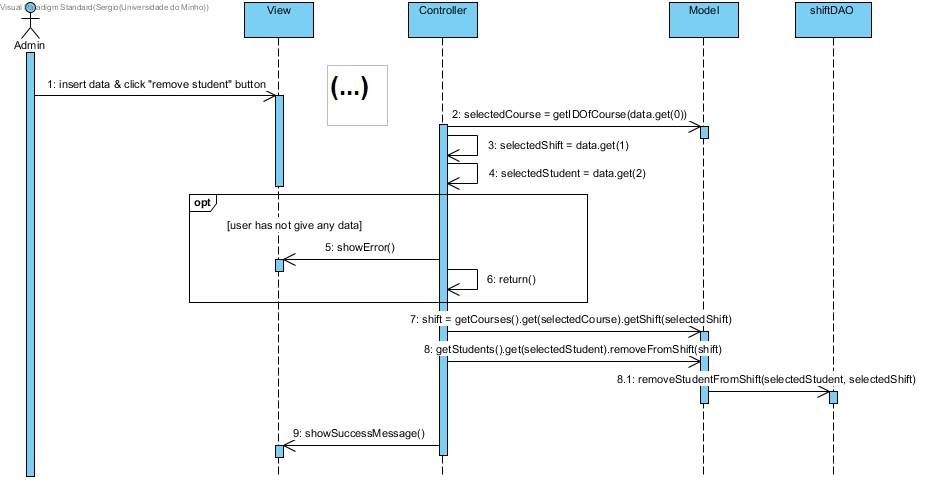
\includegraphics[width=14cm]{SEQRemoverAlunoTurno(peloAdmin)}
\caption{Diagrama de sequência para remoção de um aluno de um turno, pelo ADMIN}
\label{}
\end{figure}

\subsubsection{Ativar trocas}

\begin{figure}[H]
\centering
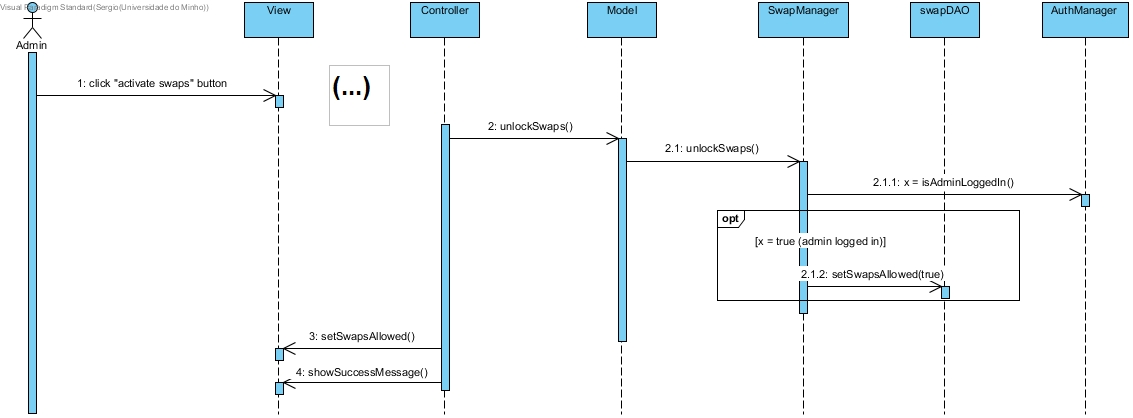
\includegraphics[width=14cm]{SEQAtivarTrocas}
\caption{Diagrama de sequência para ativação de trocas, pelo ADMIN}
\label{}
\end{figure}

\subsubsection{Desativar trocas}

\begin{figure}[H]
\centering
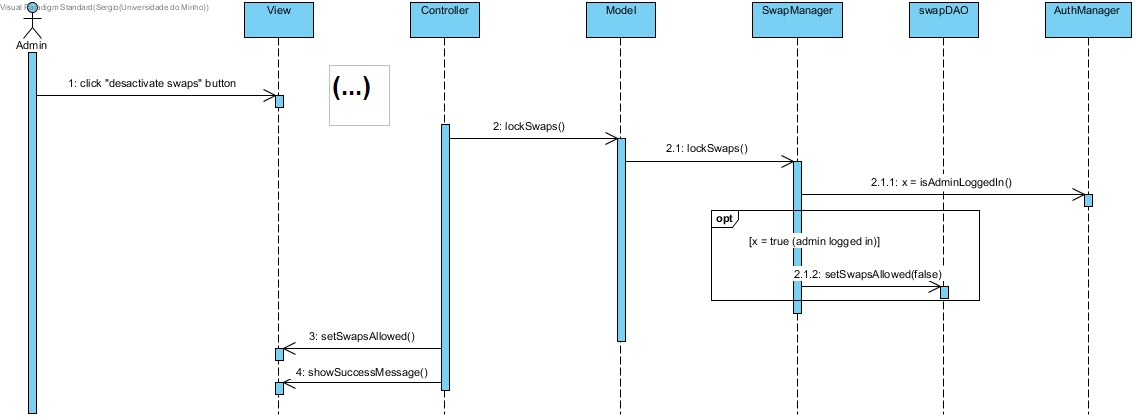
\includegraphics[width=14cm]{SEQDesativarTrocas}
\caption{Diagrama de sequência para desativação de trocas, pelo ADMIN}
\label{}
\end{figure}

\subsubsection{Efetuar login}

\begin{figure}[H]
\centering
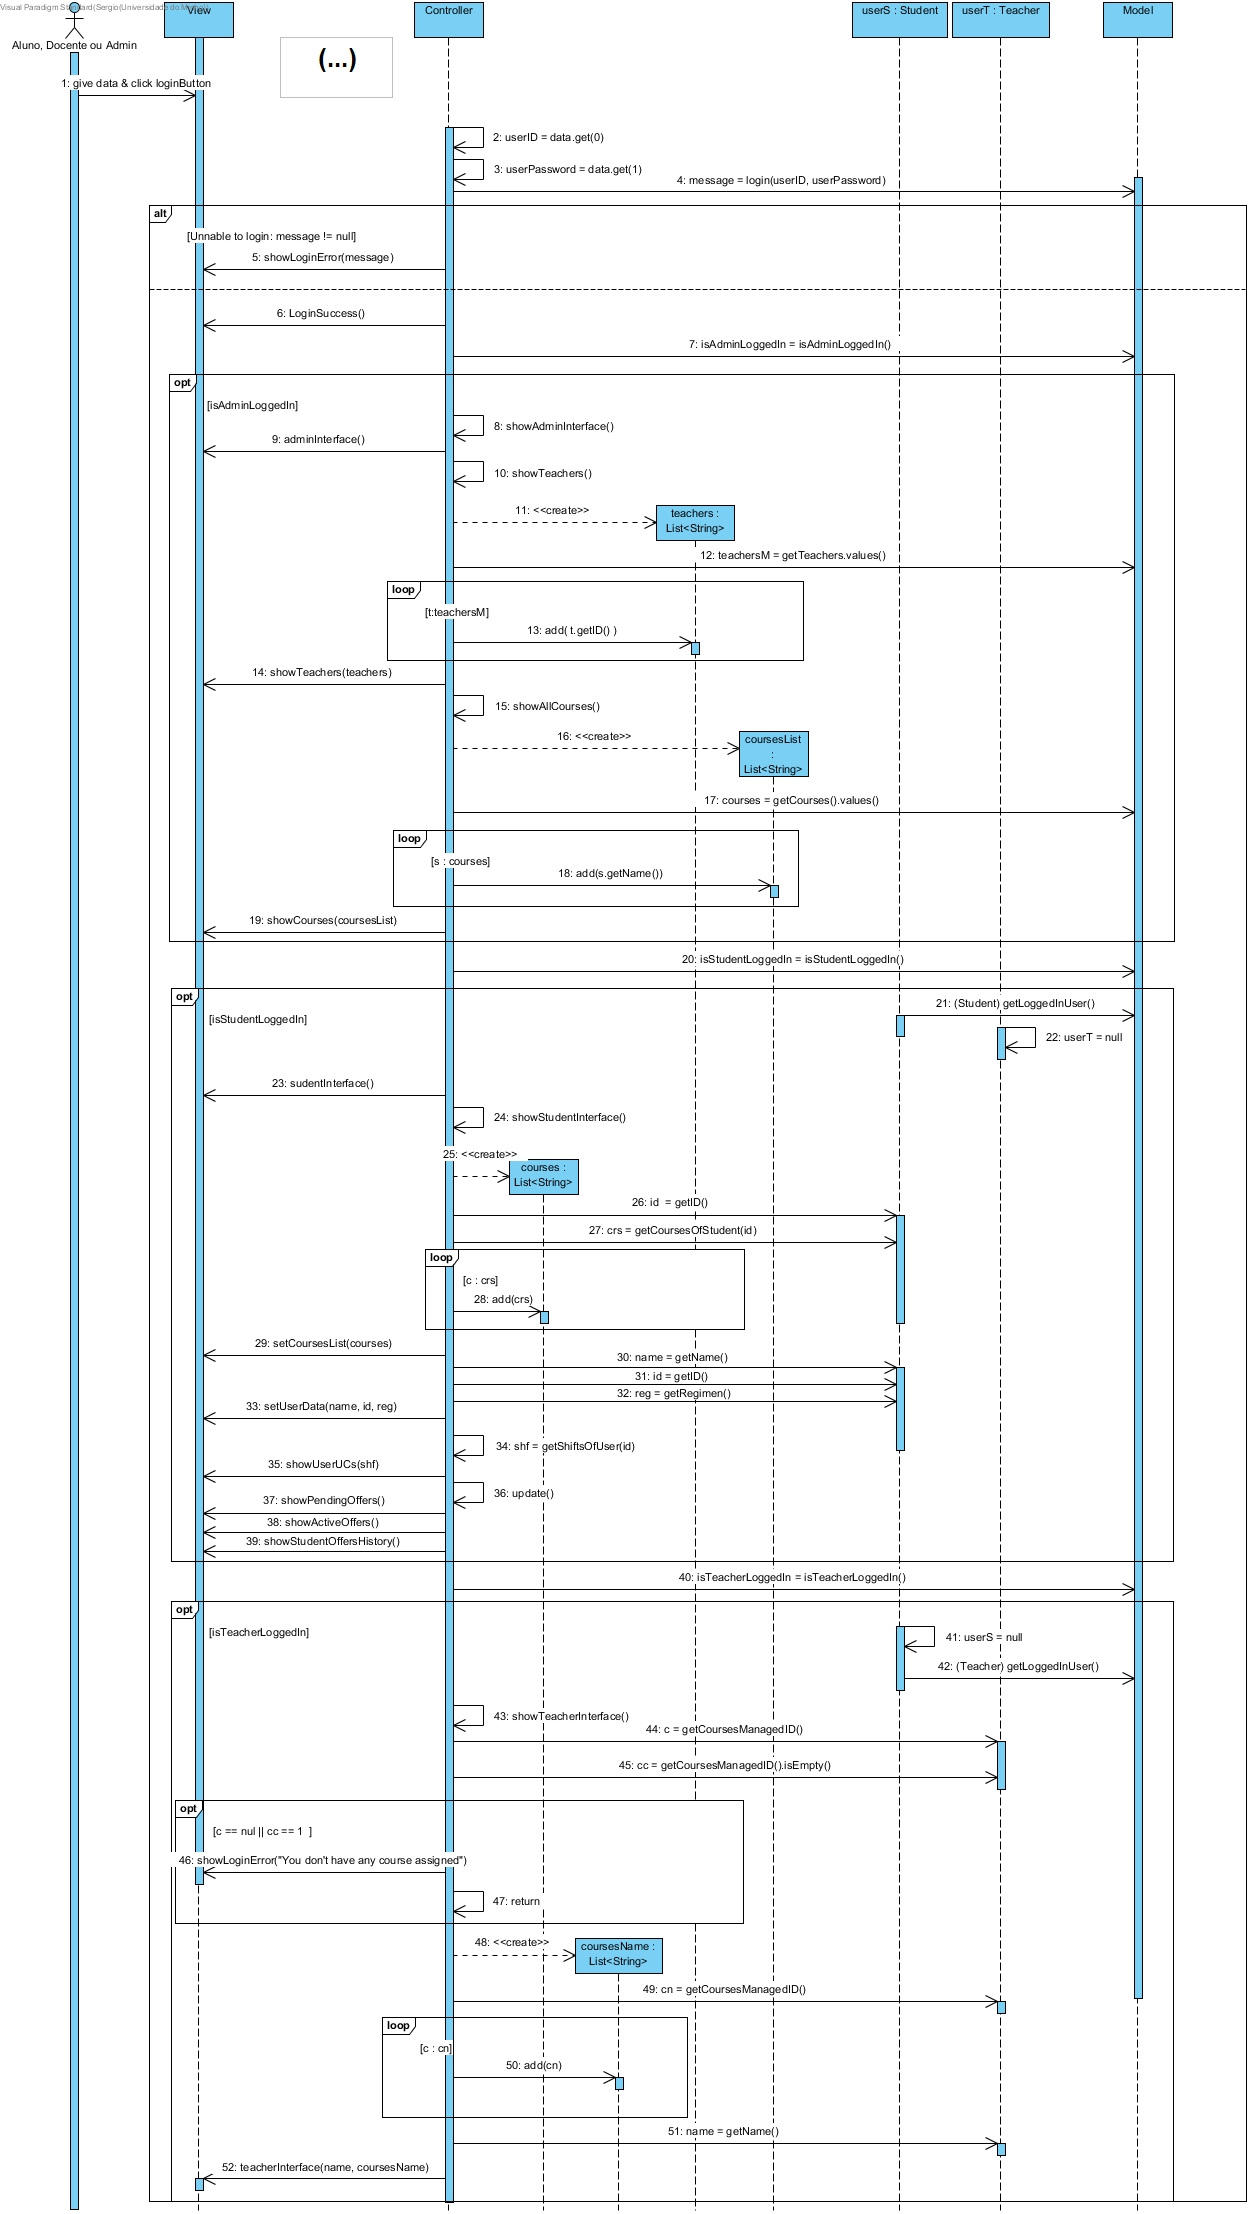
\includegraphics[height=20cm]{SEQEfetuarLogin}
\caption{Diagrama de sequência para o \emph{login} na plataforma GodSwap}
\label{}
\end{figure}

\subsubsection{Efetuar registo}

\begin{figure}[H]
\centering
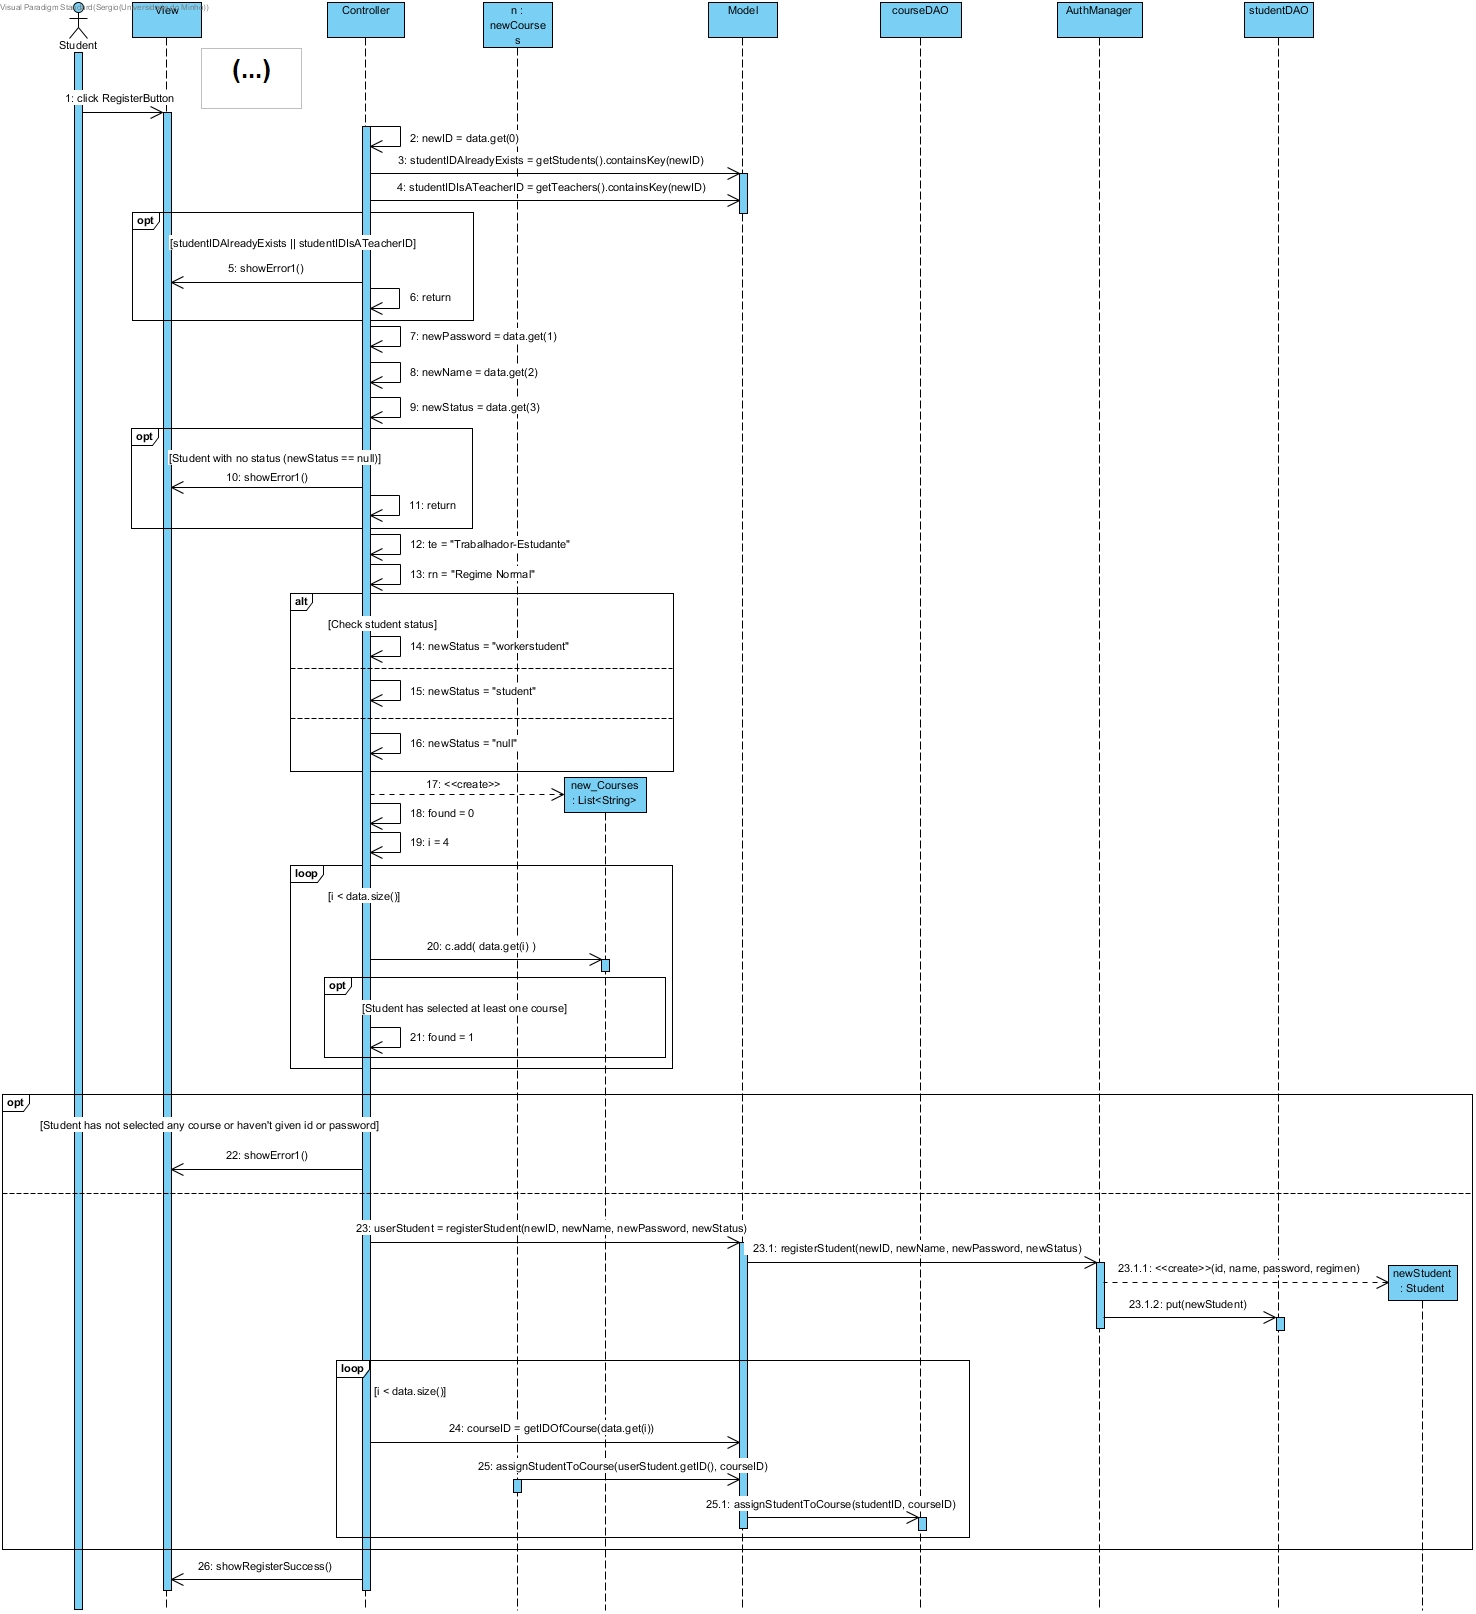
\includegraphics[width=14cm]{SEQEfetuarRegisto}
\caption{Diagrama de sequência para o registo necessário ao alunos, no início do semestre}
\label{}
\end{figure}

\subsubsection{Inscreve aluno em turno[DOCENTE]}

\begin{figure}[H]
\centering
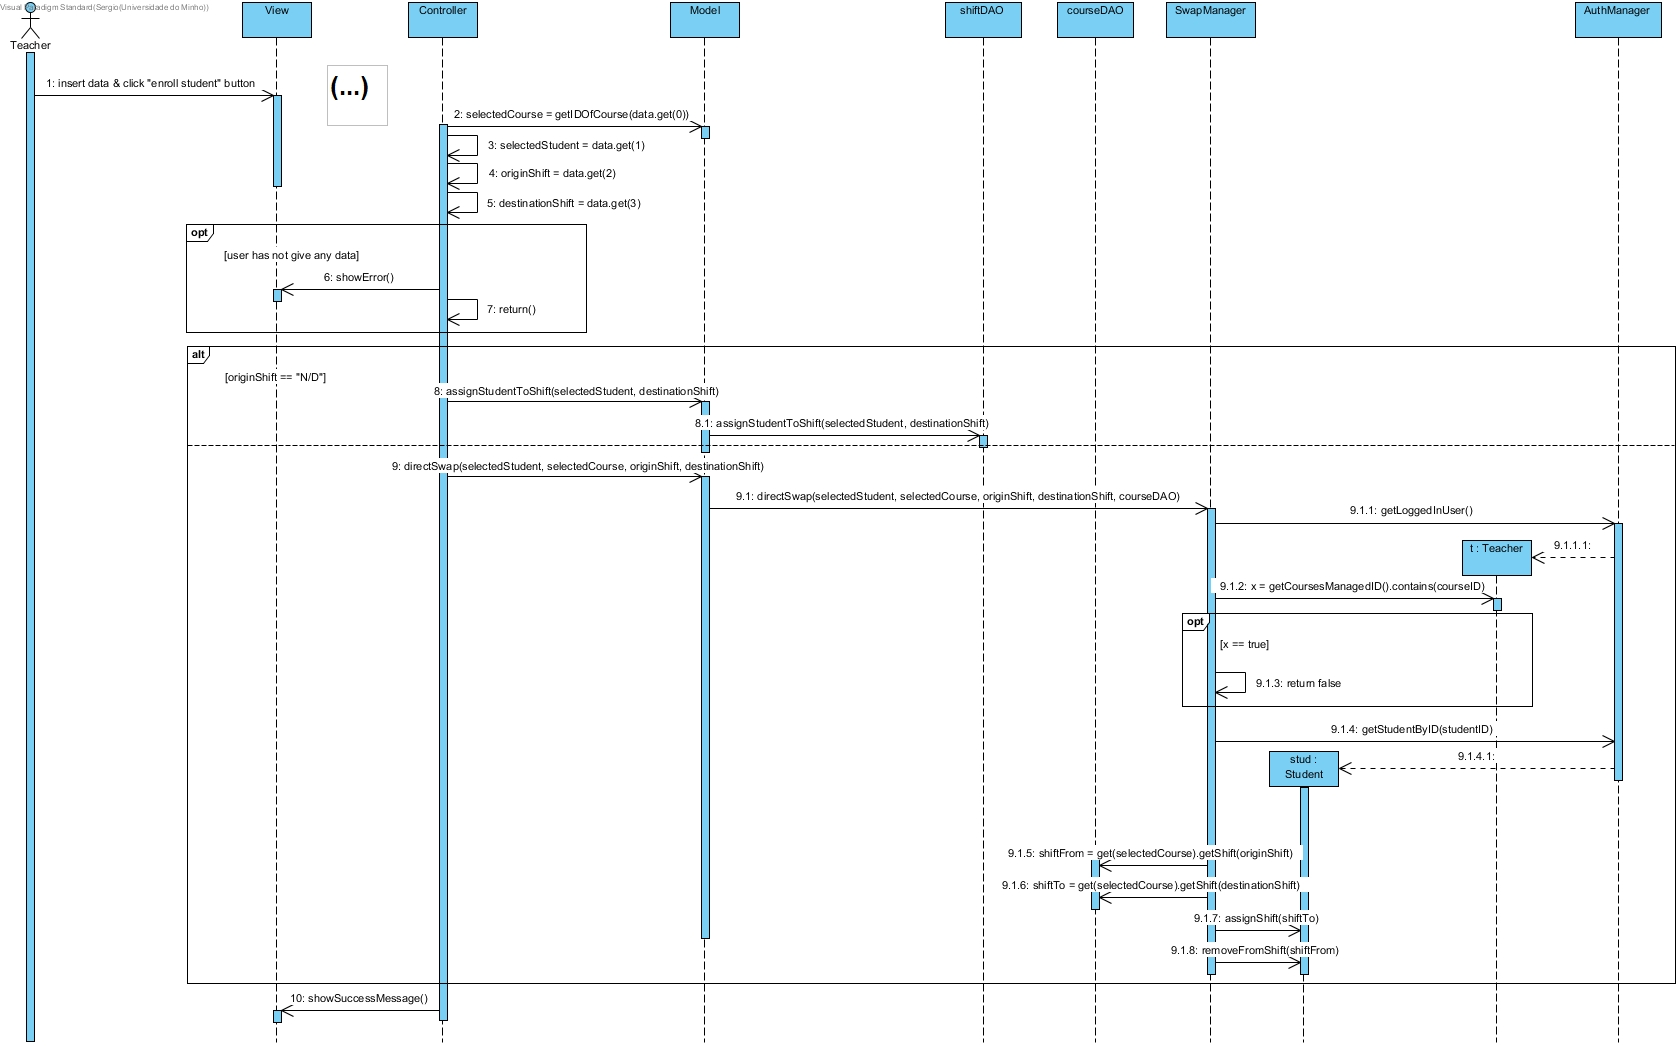
\includegraphics[width=14cm]{SEQInscreverAlunoTurno(peloDocente)}
\caption{Diagrama de sequência para a inscrição de um aluno, numa UC gerida pelo docente}
\label{}
\end{figure}

\subsubsection{Remove aluno de turno[DOCENTE]}
\begin{figure}[H]
\centering
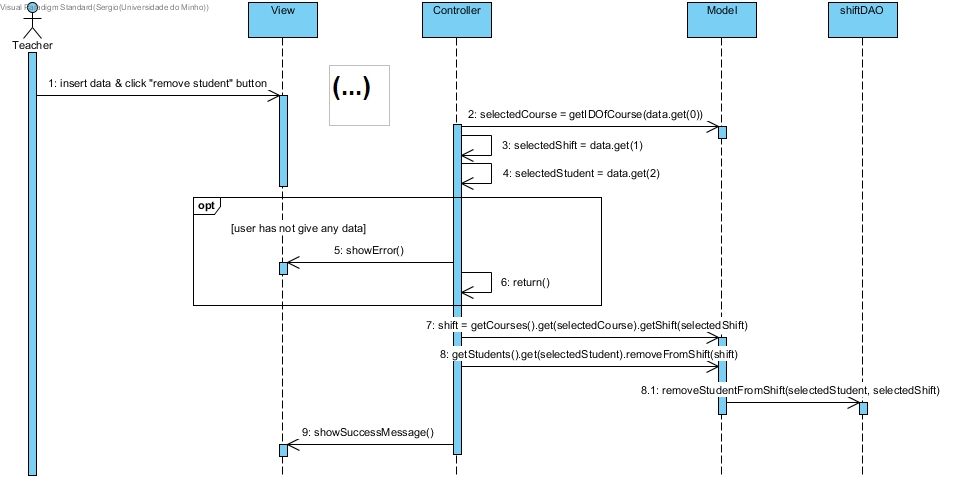
\includegraphics[width=14cm]{SEQRemoverAlunoTurno(peloDocente)}
\caption{Diagrama de sequência para remoção de um aluno, numa UC gerida pelo docente}
\label{}
\end{figure}

\subsubsection{Propor troca}

\begin{figure}[H]
\centering
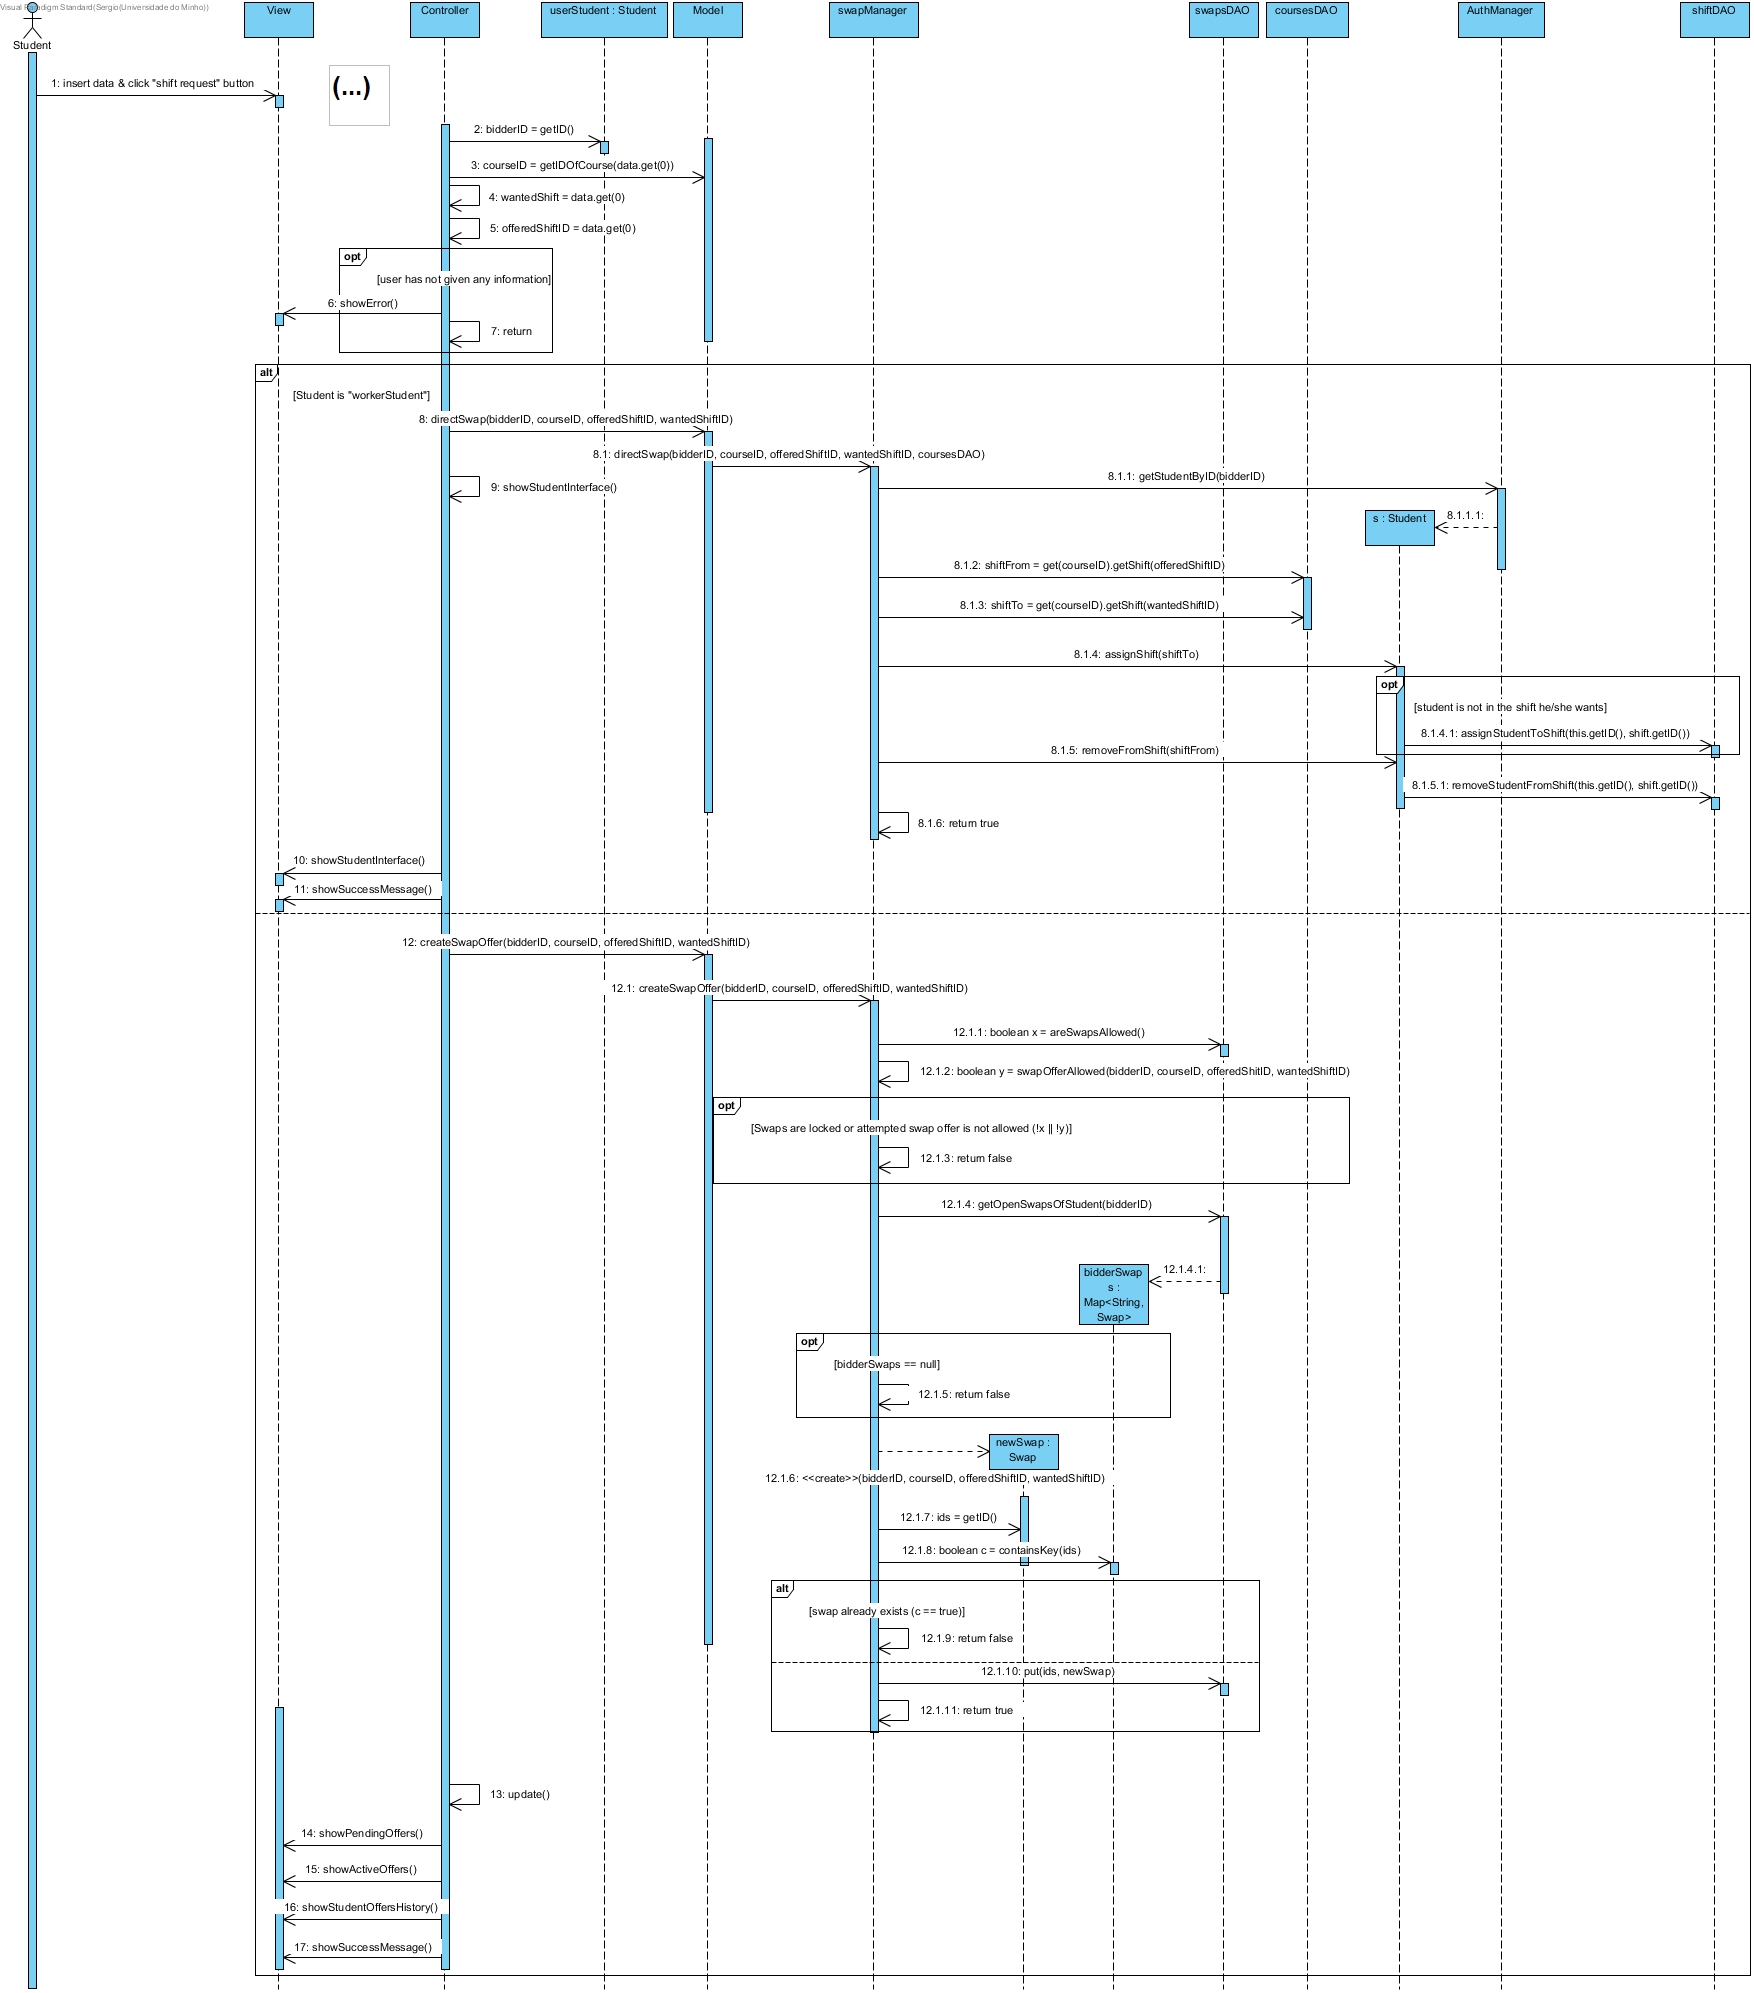
\includegraphics[width=14cm]{SEQProporTroca}
\caption{Diagrama de sequência para o lançamento de uma proposta para a bolsa}
\label{}
\end{figure}

\subsubsection{Aceitar troca}

\begin{figure}[H]
\centering
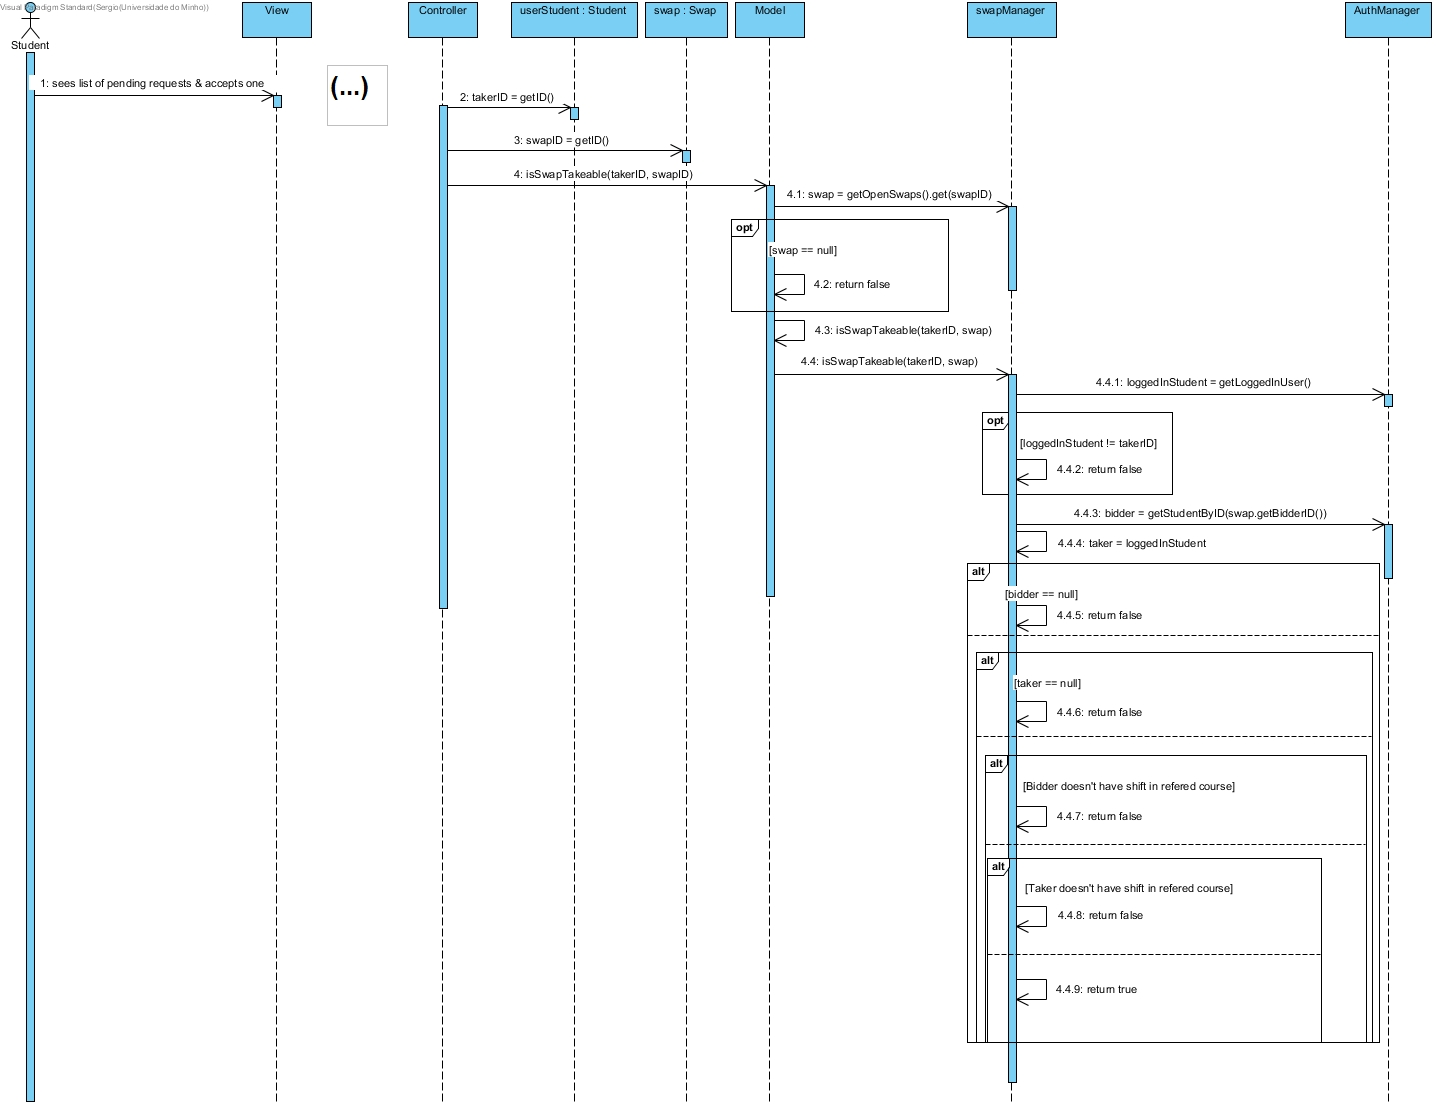
\includegraphics[width=14cm]{SEQAceitarTroca}
\caption{Diagrama de sequência para a confirmação de uma oferta de troca}
\label{}
\end{figure}

\pagebreak
\subsection{Diagramas de Máquinas de estado}
\hspace{3mm}Os diagramas de máquinas de estado modelam todos os estados possíveis que o objeto/sistema atravessa em resposta aos eventos que podem ocorrer.

\subsubsection{GODSWAP - Sistema de Gestão de Turnos}
\begin{figure}[H]
\centering
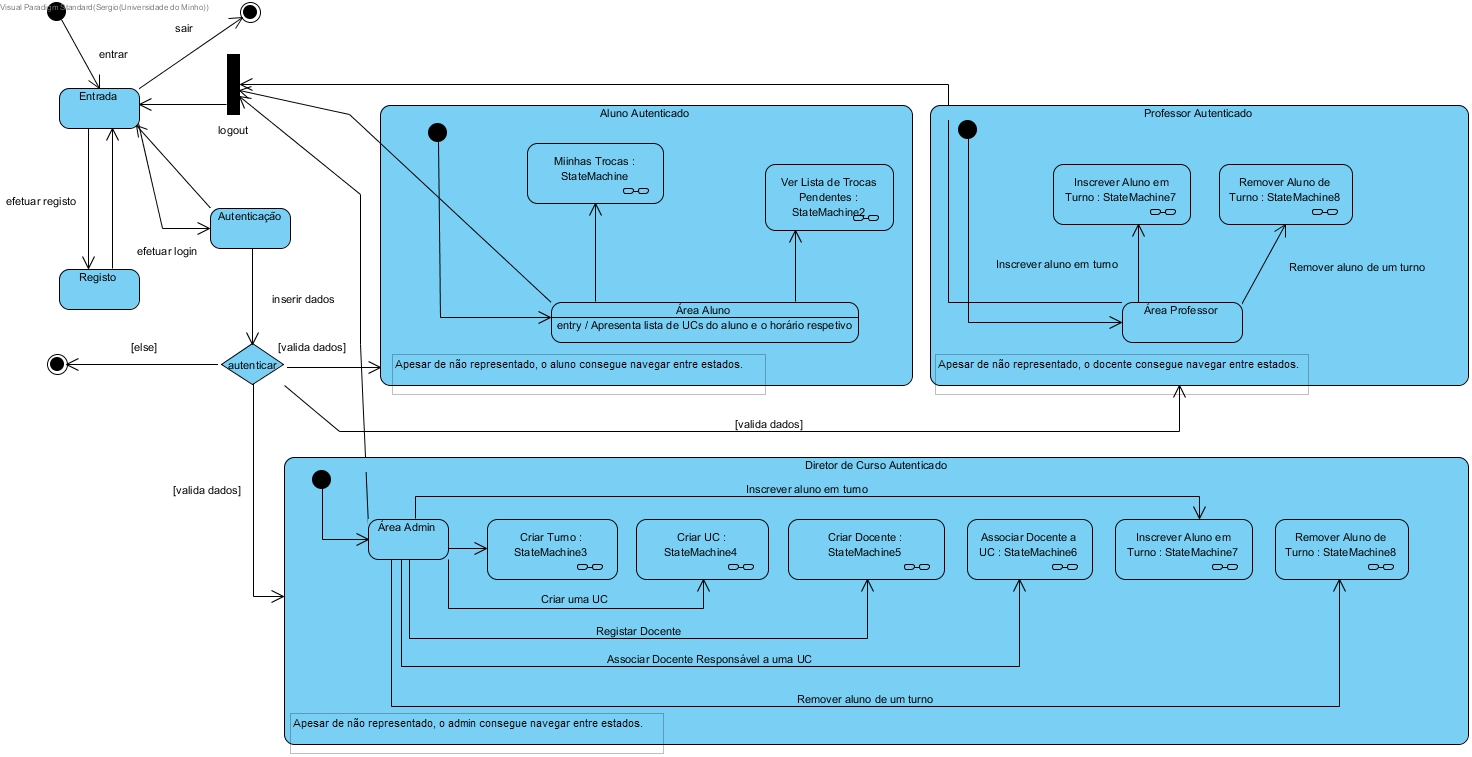
\includegraphics[width=11cm]{MEGodSwap}
\caption{GODSWAP - Sistema de Gestão de Turnos}
\label{}
\end{figure}

\subsubsection{Minhas Trocas - Aluno}
\begin{figure}[H]
\centering
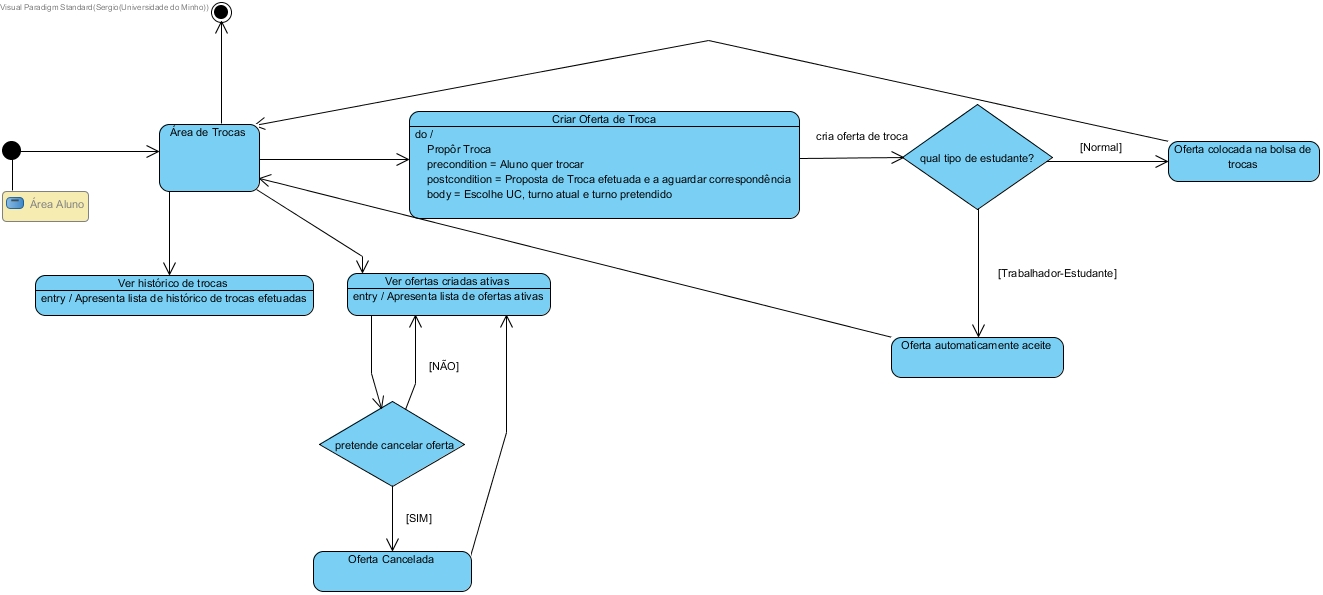
\includegraphics[width=11cm]{MEMinhasTrocas}
\caption{Secção minhas trocas, quando um aluno está logado}
\label{}
\end{figure}

\subsubsection{Ver Lista de Trocas Pendentes - Aluno}
\begin{figure}[H]
\centering
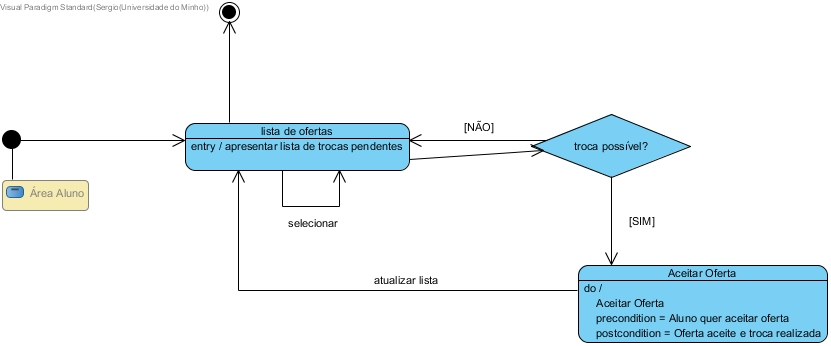
\includegraphics[width=11cm]{MEVerListadeTrocasPendentes}
\caption{Secção trocas pendentes, quando um aluno está logado}
\label{}
\end{figure}

\subsubsection{Criar Turno - DC}
\begin{figure}[H]
\centering
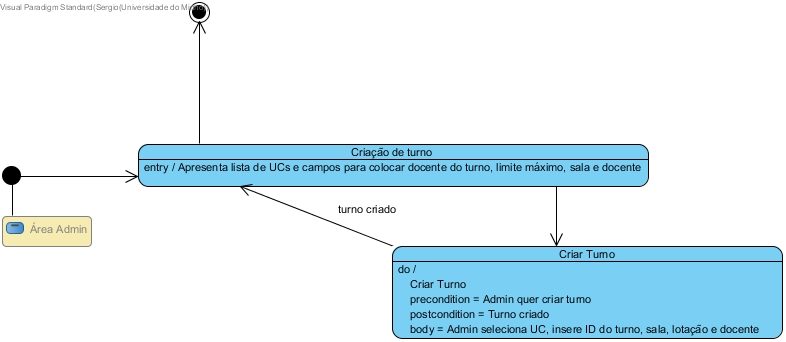
\includegraphics[width=11cm]{MECriarTurno}
\caption{Criar turno, quando o admin está logado}
\label{}
\end{figure}

\subsubsection{Criar UC - DC}
\begin{figure}[H]
\centering
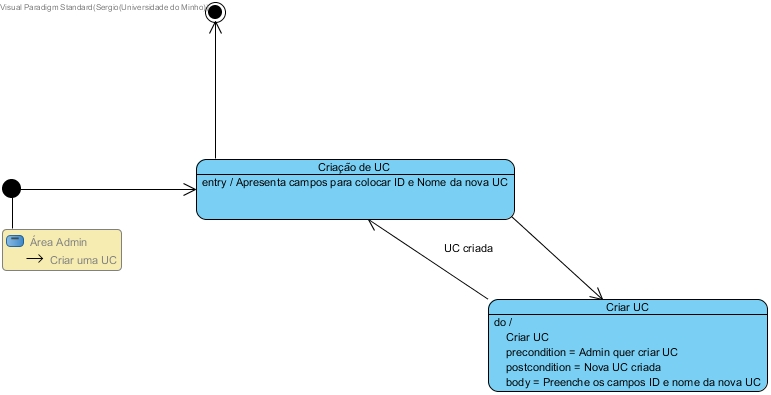
\includegraphics[width=11cm]{MECriarUC}
\caption{Criar UC, quando o admin está logado}
\label{}
\end{figure}

\subsubsection{Criar Docente - DC}
\begin{figure}[H]
\centering
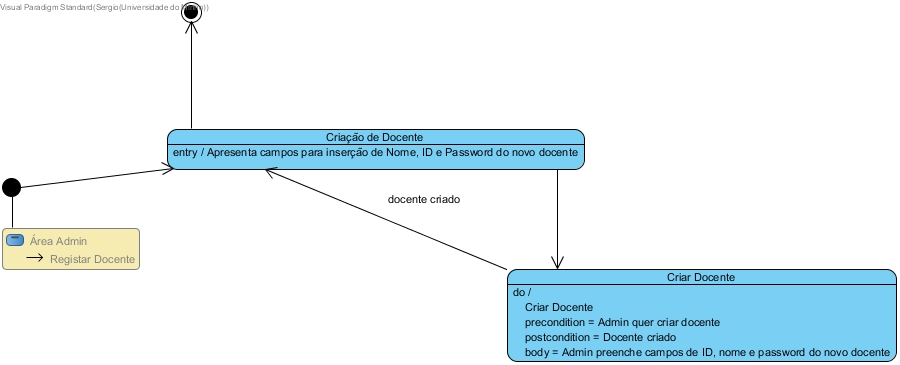
\includegraphics[width=11cm]{MECriarDocente}
\caption{Criar docente, quando o admin está logado}
\label{}
\end{figure}

\subsubsection{Associar Docente a UC - DC}
\begin{figure}[H]
\centering
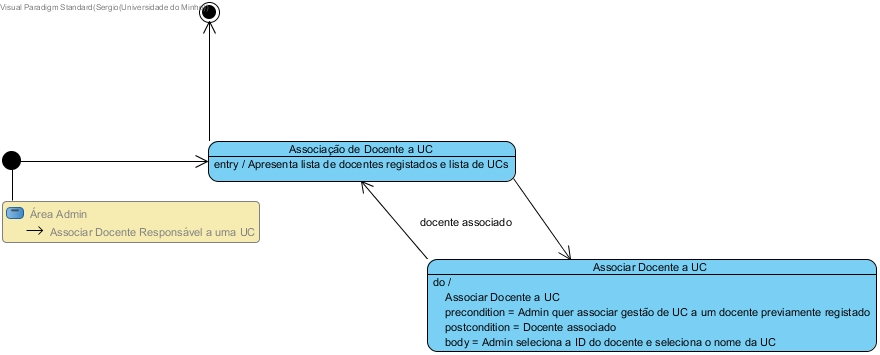
\includegraphics[width=11cm]{MEAssociarDocenteaUC}
\caption{Associar docente a UC, quando o admin está logado}
\label{}
\end{figure}

\subsubsection{Inscrever Aluno em Turno - DC/Docente}
\begin{figure}[H]
\centering
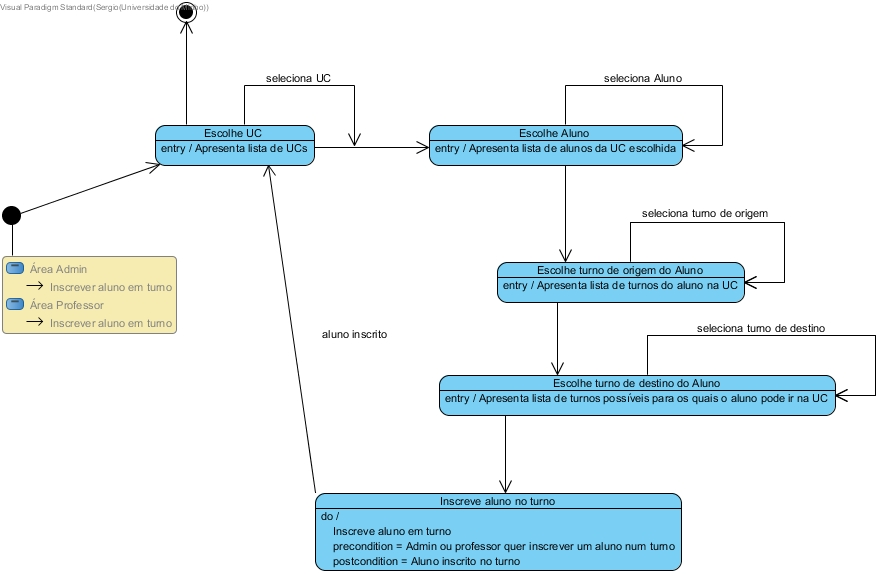
\includegraphics[width=11cm]{MEInscreveralunoemturno}
\caption{Inscrever aluno em turno, quando o admin ou o docente estão logados}
\label{}
\end{figure}

\subsubsection{Remover Aluno de Turno - DC/Docente}
\begin{figure}[H]
\centering
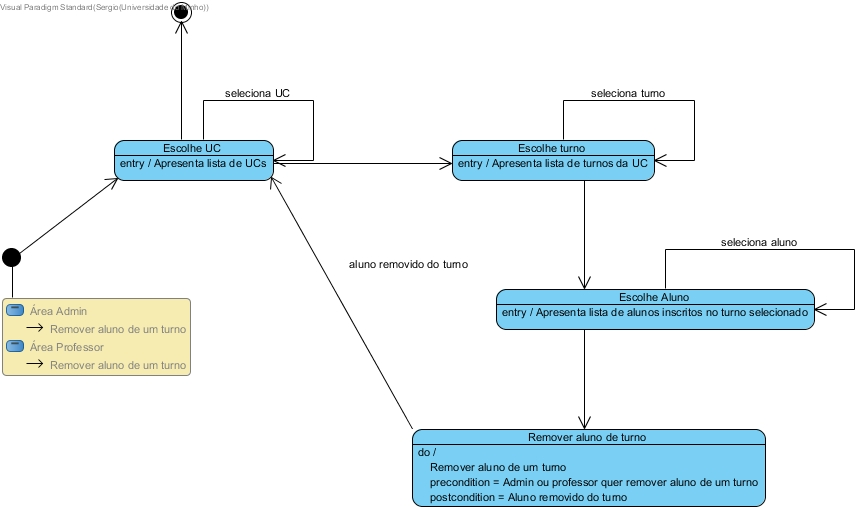
\includegraphics[width=11cm]{MERemoveralunodeturno}
\caption{Remover aluno de turno, quando o admin ou o docente estão logados}
\label{}
\end{figure}

\clearpage
\subsection{Diagramas de Atividade}
\hspace{3mm}

Quanto aos diagramas de atividade, decidimos que a criação/aceitação de ofertas de troca de turno é a funcionalidade que mais beneficia do recurso a este tipo de diagrama. Sendo esta funcionalidade o componente central da aplicação, e a ação de mais importância realizada pelo utilizador, tentamos demonstrar a sequência respetiva de ações de uma maneira fácil de compreender.

\subsubsection{Criar Troca}
\begin{figure}[H]
\centering
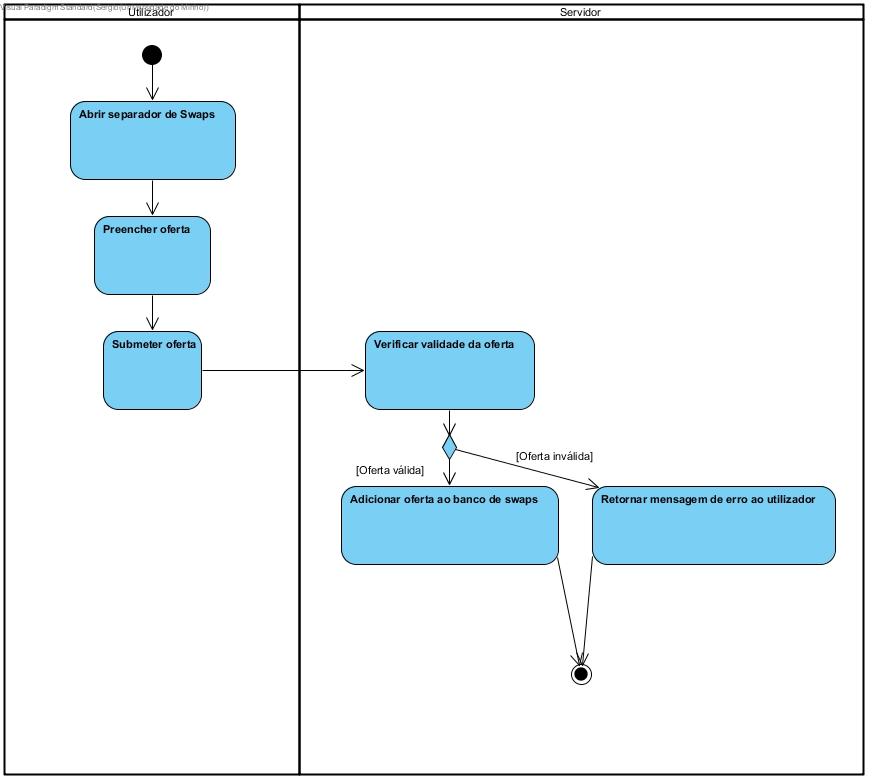
\includegraphics[width=12cm]{AtividadeCriarTroca.jpg}
\caption{Diagrama de atividade da funcionalidade "Criar Troca"}
\label{}
\end{figure}

\subsubsection{Aceitar Troca}
\begin{figure}[H]
\centering
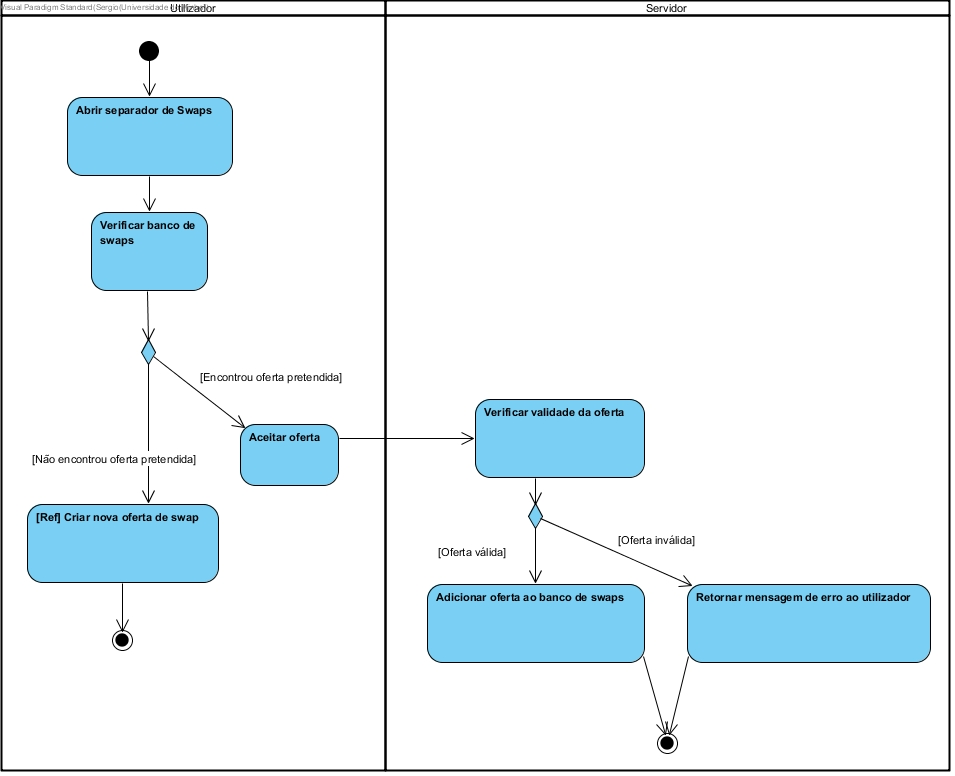
\includegraphics[width=12cm]{AtividadeAceitarTroca.jpg}
\caption{Diagrama de atividade da funcionalidade "Aceitar Troca"}
\label{}
\end{figure}

\clearpage
\subsection{Diagrama de Packages}
\hspace{3mm}Nesta fase, representamos os diferentes packages do trabalho, assim como as relações existentes entre estes.

\begin{figure}[H]
\centering
\includegraphics[width=14cm]{DiagramaPackages}
\caption{Diagrama de Packages}
\label{}
\end{figure}

\clearpage
\subsection{Diagrama de Instalação}
\hspace{3mm}O Diagrama de instalação descreve os componentes de hardware e software representando, assim, a configuração e a arquitetura do GODSWAP.

\begin{figure}[H]
\centering
\includegraphics[width=14cm]{DiagramaInstalacao}
\caption{Diagrama de Instalação}
\label{}
\end{figure}


\subsection{Prototipagem da Interface Gráfica}
\hspace{3mm} Segue-se a prototipagem simples da interface, realizada na primeira fase do projeto.

\subsubsection{Login/Registo}
\begin{figure}[H]
\centering
\includegraphics[width=11cm]{interface_1}
\caption{Área de Login e de Registo}
\label{}
\end{figure}


\subsubsection{Minha Área}
\begin{figure}[H]
\centering
\includegraphics[width=11cm]{interface_2}
\caption{Apresentação do horário do aluno}
\label{}
\end{figure}

\subsubsection{Minhas Trocas}
\begin{figure}[H]
\centering
\includegraphics[width=11cm]{interface_3}
\caption{Área onde o aluno poderia criar uma oferta de troca e visualizar o histórico de trocas}
\label{}
\end{figure}

\subsubsection{Ver Lista de Trocas Pendentes}
\begin{figure}[H]
\centering
\includegraphics[width=11cm]{interface_4}
\caption{Implementação da bolsa de trocas, visualmente falando}
\label{}
\end{figure}

\clearpage
\subsection{Interface Gráfica}
\hspace{3mm} Foram necessários ajustes em relação ao protótipo apresentado anteriormente, que foram feitos aquando da concretização da mesma em JAVA, no entanto, verifica-se que o grupo foi, ainda assim, fiel ao modelo inicial.

\begin{figure}[H]
\centering
\includegraphics[width=13.5cm]{IjanelaInicial}
\caption{Janela Inicial}
\label{}
\end{figure}

\begin{figure}[H]
\centering
\includegraphics[width=13.5cm]{Ilogin}
\caption{Janela de Login}
\label{}
\end{figure}

\begin{figure}[H]
\centering
\includegraphics[width=13.5cm]{IRegisto}
\caption{Janela de Registo}
\label{}
\end{figure}

\begin{figure}[H]
\centering
\includegraphics[width=13.5cm]{IMinhaAreaALUNO}
\caption{Área de \textbf{Aluno}}
\label{}
\end{figure}

\begin{figure}[H]
\centering
\includegraphics[width=13.5cm]{IminhastrocasALUNO}
\caption{Trocas do \textbf{Aluno}}
\label{}
\end{figure}

\begin{figure}[H]
\centering
\includegraphics[width=13.5cm]{ItrocaspendentesALUNO}
\caption{Trocas pendentes no Sistema}
\label{}
\end{figure}

\begin{figure}[H]
\centering
\includegraphics[width=13.5cm]{IgestaoDOCENTE}
\caption{O \textbf{docente} responsável consegue inscrever alunos em turnos e removê-los, na sua UC}
\label{}
\end{figure}

\begin{figure}[H]
\centering
\includegraphics[width=13.5cm]{IgestaoADMIN}
\caption{O \textbf{DC} consegue inscrever alunos em turnos e removê-los}
\label{}
\end{figure}

\begin{figure}[H]
\centering
\includegraphics[width=13.5cm]{IcriarADMIN}
\caption{O \textbf{DC} pode criar turnos e unidades curriculares}
\label{}
\end{figure}

\begin{figure}[H]
\centering
\includegraphics[width=13.5cm]{IdocentesADMIN}
\caption{O \textbf{DC} pode criar docentes e associá-los a unidades curriculares}
\label{}
\end{figure}

\begin{figure}[H]
\centering
\includegraphics[width=13.5cm]{IfuncionalidadesADMIN}
\caption{Funcionalidades avançadas do \textbf{DC}}
\label{}
\end{figure}


\subsection{Passagem para Data Access Objects}

Previamente, esta informação era guardada nas seguintes estruturas:

\begin{enumerate}
   \item Classe \emph{AuthManager}
   \begin{itemize}
     \item HashMap\textless String, Student\textgreater registeredStudents 
     \item HashMap\textless String, Teacher\textgreater registeredTeachers (ambos guardam informação relativo a utilizadores registados no formato ID de utilizador -\textgreater utilizador)
   \end{itemize}
   \item Classe \emph{Model}
   \begin{itemize}
       \item HashMap\textless String, Course\textgreater courses (guarda informação relativa às UCs existentes no formato ID de UC -\textgreater UC)
   \end{itemize}
   \item Classe \emph{SwapManager}
   \begin{itemize}
       \item HashMap\textless String, HashMap\textless String, Swap\textgreater swapsByStudentID (guarda informação relativa a trocas de turnos entre alunos no formato ID de aluno -\textgreater Mapa de de trocas (ID de troca -\textgreater troca)
   \end{itemize}
   \item Classe \emph{Course}
   \begin{itemize}
       \item HashMap\textless String, Shift\textgreater shifts (guarda informação relativa a turnos no formato ID de turno -\textgreater turno)
   \end{itemize}
   \item Classe {Student}
   \begin{itemize}
       \item HashMap\textless String, Shift\textgreater shifts (guarda informação relativa aos turnos em que um aluno está inscrito)
   \end{itemize}
\end{enumerate}

Depois da criação dos DAOs respetivos, as classes passaram a usar as seguintes estruturas:

\begin{enumerate}
   \item Classe \emph{AuthManager}
   \begin{itemize}
     \item studentDAO
     \item studentDAO
   \end{itemize}
   \item Classe \emph{Model}
   \begin{itemize}
       \item courseDAO
   \end{itemize}
   \item Classe \emph{SwapManager}
   \begin{itemize}
       \item swapDAO
   \end{itemize}
   \item Classe \emph{Course}
   \begin{itemize}
       \item shiftDAO (mais especificamente, o método \emph{shiftDAO.getShiftsOfCourse})
   \end{itemize}
   \item Classe {Student}
   \begin{itemize}
       \item shiftDAO (mais especificamente, \emph{shiftDAO.getShiftsOfStudent})
   \end{itemize}
\end{enumerate}

\clearpage
Foi feito especial cuidado de maneira a que os DAOs apenas fossem utilizados nestas classes. Os métodos continuam a retornar a mesma informação que anteriormente, apenas se tendo mudado a estrutura que os guarda, de maneira invisível para os métodos que fazem uso destas classes, comprovando a modularidade da aplicação.

Estes DAOs foram elaborados tendo em mente o seguinte esquema de base de dados elaborado com a ajuda do \emph{MySQL Workbench}:

\begin{figure}[h]
\caption{Esquema da base de dados da aplicação GodSwap}
\centering
\includegraphics[width=0.8\textwidth]{database}
\end{figure}

\subsection{Carregamento de dados JSON}
Para carregar os dados relativos às UCs existentes no curso, assim como dados de alunos para testes, foi criada a classe \emph{CustomJSONParser}, que utiliza o pacote \emph{JSON.simple} para \emph{Java}.

Foi utilizado o serviço \emph{Mockaroo} para gerar dados aleatórios de alunos para testes, como recomendado pelos docentes.

Nesta classe foram também incluídos alguns métodos auxiliares que permitem popular a base de dados com a informação presente nos ficheiros JSON.

\pagebreak
\section{Conclusões}
\hspace{3mm}Inicialmente, para a primeira fase deste projeto, foram desenvolvidos o modelo de domínio, o modelo de \textit{Use Cases}e respetivas especificações, para além do protótipo de interface gráfica. O grupo tentou identificar todas as necessidades a que o sistema deveria dar resposta e respetivos utilizadores, tendo a primeira fase sido concluída com sucesso.

De seguida, e tal como pedido para a segunda fase do projeto, criaram-se os restantes diagramas, que permitiriam à equipa um desenvolvimento mais capaz e acelerado, apesar da demora inicial que o desenho destes diagramas impõe. Desta feita, surgiram diagramas de Classes, de Sequência, de Máquinas de Estado, de Atividades, de Packages e, por fim, de Instalação.

Iniciada a programação do programa especificado, de acordo com o padrão MVC, o grupo decidiu utilizar \textit{Consumers}, solução que se apresentou interessante e permitiu alargar os conhecimentos em Java. Como seria de esperar, apesar de se acreditar que todos os Diagramas respondiam às necessidades encontradas, surgiram problemas que não haviam sido antevistos na fase inicial. Naturalmente, procedeu-se ao ajuste e correção dos Diagramas necessários, sendo que os de Sequência foram os que apresentaram a maior parte das alterações à medida que o projeto ficava concluído. Assim, tornou-se bem claro da relação estreita que é estabelecida entre estes diagramas e o código necessário ao programa.

Adicionalmente, e como o grupo pretendeu fazer um trabalho completo, procedeu-se à troca das estruturas de dados temporárias utilizadas no desenvolvimento (\textit{Hashmaps} e \textit{Arrays}, principalmente) por uma Base de Dados, tal como sugerido nos diversos diagramas. Foi necessário algum esforço para criar todos os \textit{DAOs}, mais que o projetado inicialmente, pois o grupo nunca havia lidado com este tipo de padrão para acesso de dados. Mais ainda, e não satisfeito com o trabalho elaborado, tomou-se a decisão de desenvolver uma atribuição automática de turnos, como sugerido pelos docentes, apesar do pouco tempo para o término. Assim, a distribuição automática foi feita, não sendo a melhor, uma vez que podem ocorrer algumas (não frequentes) sobreposições, que poderiam ser reparadas com mais algum tempo que o grupo nao teve.

Por fim, foi desenvolvida a interface gráfica, que ficou próxima àquilo que projetado inicialmente em termos de funcionalidade, à exceção do menu inicial.

O grupo considera que o trabalho foi extenso e exigente, tendo-se esforçado para cumprir com todos os pontos pedidos, com vista à obtenção da nota máxima, tal como é sempre o desejo dos seus membros. Alguns diagramas foram considerados mais importantes que outros, sendo que ficaram claras as implicações a nível de flexibilidade de desenvolvimento que um ou outro diagrama pode implicar, tendo sido adquiridas boas bases para futuras aplicações.
\label{sec:4}

\hspace{3mm}
\end{document}
